% paper.tex -- seminar paper draft.
% GRADE-REPORT RESPONSE 2026-09-22 (seminar_grade_report.md; docs/decisions/grade-report-response.md).
% Every regression and summary table is now GENERATED: main.R's build_paper_tables() writes the
% tabular blocks to paper/tables/*.tex (plus auto_notes.tex for the dropped-coefficient note
% macros) and this file \input{}s them inside hand-written floats. Numbers in the prose were
% re-verified against the same run's outputs/*.csv. Additions: Table 2 columns (3)-(4) (saturated
% FE and quartile-binned DDD), Table 4 blocks for outcome coding and inference (wild bootstrap,
% permutation test), the falsification subsection, the child-age heterogeneity subsection and its
% table/figure, the occupation-level first stage and the appendix table of the forty scores.
% EDITORIAL PASS 2026-09-22 (paper/notes/editorial-audit-2026-09-22.md, section M). Step 1 was
% text-only. Step 2 added six artifacts from a full pipeline re-run the same day, all in outputs/:
%   - ddd_hours_unswapped.csv (DDD on the 30 unswapped occupations), ddd_hours_ex2023.csv and
%     intensive_margin_ex2023.csv (DDD and DiD without 2023), ddd_hours_twoway_cluster.csv;
%   - wfh_share_by_year.csv (Israeli realized-WFH shares, Introduction);
%   - absence_by_exposure_quartile_{by_quartile,by_cell}.csv (Limitations footnote);
%   - hours_dose_response_data.csv gained a mean_exposure column (the Q4-Q1 scaling in 5.2).
% The per-SD / per-IQR scalings in 5.2 and Table 2 come from mde_hours.csv's regressor_sd /
% regressor_iqr columns, which pre-date the audit. Every pre-existing CSV reproduced byte for byte.
% Step 3 (same day) added four Crossref-verified citations (bib header lists them), the earnings
% sentence in 3.1 (the codebook has no earnings amount), and single-spaced the regression tables.
% The only remaining "% TODO(<item>)" comment is J/D11: the Conclusion and the fixed date.
% EVERY hours-derived figure below was re-verified 2026-09-21 against a full pipeline re-run after
% the hours population was harmonized across survey years (docs/decisions/hours-population-
% harmonization.md, Checkpoint 13) and the Lee-bounds selection rate was redefined on the
% observed-hours sample. Do NOT compare any hours number here against an outputs/ CSV from before
% that date. Employment-margin figures, the WFH-exposure construction and Table 1's non-hours rows
% are unaffected and still carry their original provenance below.
% Provenance of the numbers, verified 2026-09-19 against a full pipeline re-run:
%   - most figures come from paper/notes/results_digest.md (2026-09-15), which attributes each to
%     a file in outputs/;
%   - Table 1 comes from outputs/descriptive_table_continuous.csv and _categorical.csv, which
%     post-date the digest and are not listed in it;
%   - the hours-DDD constant (30.51) comes from outputs/ddd_hours_table.csv, which the digest's
%     own table omits;
%   - a handful of values (the MDEs, both Imbens-Manski intervals, the joint Wald tests, the
%     two-sample z-tests, the 1.9% panel share) are console-only: reproducible by re-running the
%     pipeline but written to no file. See results_digest.md section 7.
% Compiled with pdflatex + bibtex (four passes); bibliography: paper/references.bib.
\documentclass[12pt,a4paper]{article}

\usepackage[utf8]{inputenc}
\usepackage{lmodern} % scalable Type 1 T1 fonts; without this, fontenc pulls EC bitmap (Type 3) fonts
\usepackage[T1]{fontenc}
\usepackage{amsmath}
\usepackage{booktabs}
\usepackage{threeparttable}
\usepackage{graphicx}
\usepackage{geometry}
\geometry{margin=2.5cm}
\usepackage{setspace}
\onehalfspacing
\usepackage[authoryear,round]{natbib}
\usepackage{xcolor} % draft-conclusion flag
\usepackage{hyperref}
\hypersetup{colorlinks=true, linkcolor=blue, citecolor=blue, urlcolor=blue}

\newcommand{\sym}[1]{\ensuremath{^{#1}}}
\newcommand{\Mother}{\text{Mother}}
\newcommand{\Post}{\text{Post}}
\newcommand{\WFH}{\text{WFH\_Exposure}}
% Generated by main.R (scripts/export_paper_tables.R): one \newcommand per table-note
% sentence about coefficients dropped for collinearity. Never edit by hand.
% Generated by scripts/export_paper_tables.R from a pipeline run. Do not edit by hand.
\newcommand{\autonoteHours}{No coefficient is dropped for collinearity in any column.}
\newcommand{\autonoteSubgroup}{The Arab-women DiD drops the religion category `other', constant on that sample; the Arab-women DDD drops the religion category `other', constant on that sample; no other column drops a coefficient.}
\newcommand{\autonoteChildAge}{No coefficient is dropped for collinearity in any column.}
\newcommand{\autonoteExtensive}{No coefficient is dropped for collinearity in any column.}


\title{Did Remote Work Narrow the Motherhood Penalty?\\
\large Evidence on the Intensive Margin from Israeli Labor Force Survey Microdata, 2017--2023}
\author{Inbal Moryles \and Nitzan Zacharia}
\date{Seminar paper draft --- \today}

\begin{document}

\begin{titlepage}
    \centering

    {\large \textbf{Tel Aviv University}\par}
    \vspace{0.3cm}
    {\large \textbf{Faculty of Social Sciences}\par}
    \vspace{0.3cm}
    {\large \textbf{The Eitan Berglas School of Economics}\par}

    \vspace{1.5cm}

    {\large \textbf{Seminar in Topics in Labor Economics and the Economics of Education}\par}

    \vspace{3cm}

    {\LARGE \textbf{Did Remote Work Narrow the Motherhood Penalty?}\par}
    \vspace{0.5cm}
    {\large \textbf{Evidence on the Intensive Margin from Israeli Labor Force Survey
    Microdata, 2017--2023}\par}

    \vspace{3cm}

    {\large \textbf{Submitted to: Prof.\ Analia Schlosser}\par}

    \vspace{2cm}

    {\large \textbf{Submitted by:}\par}
    \vspace{0.5cm}
    {\large Inbal Moryles \quad (ID: 212047195)\par}
    \vspace{0.2cm}
    {\large Nitzan Zacharia \quad (ID: 206539496)\par}

    \vfill

    % TODO(J/D11): replace \today with the fixed submission date when the Conclusion is written.
    {\large \textbf{Submission Date:} \today\par}

\end{titlepage}

% Contents page. tocdepth 2 pins the listing to sections and subsections: the \paragraph units in
% the Literature Review, Results and Limitations sit at level 4 and stay out. The \begingroup
% wrapper prints entries in black rather than hyperref's blue while leaving them clickable, and
% restores linkcolor=blue for the cross-references and citations in the body.
\setcounter{tocdepth}{2}
\begingroup
\hypersetup{linkcolor=black}
\tableofcontents
\endgroup
\newpage

\begin{abstract}
\noindent
\citet{harrington2025} ask whether the post-pandemic rise of work from home (WFH) reduced the
motherhood penalty in the United States. This paper takes that question to Israel and to the
intensive margin. Using Central Bureau of Statistics (CBS) Labor Force Survey microdata on women
aged 25--59 in 2017--2019 and 2021--2023, we estimate difference-in-differences (DiD) and
triple-differences (DDD) models of usual weekly hours for mothers relative to childless women, with
the COVID-19-driven shift to remote work as the ``post'' period and an Israeli-calibrated
occupational WFH-exposure index as the third difference. Employed mothers' hours did not change on
average ($\Mother \times \Post = 0.23$, SE $0.18$). The effect is instead \emph{confined} to
teleworkable work: the triple interaction is $3.22$ hours per unit of exposure (SE $1.02$),
about $1.8$ hours a week between the most and least teleworkable quartiles of occupations, while
the implied change at zero exposure is if anything negative. The estimate is significant at the
$1\%$ level on the analytic occupation-clustered standard error, at the $5\%$ level under a
permutation test that reassigns exposure across occupations ($p = 0.032$), and at the $10\%$
level under a wild cluster bootstrap ($p = 0.056$). It is unchanged under a fully saturated
fixed-effects specification, survives a generalized trimming-bounds correction for selection into
the estimation sample (95\% confidence interval for the identified set $[1.02, 5.32]$), and is
largest for mothers of children under five and smallest for mothers of teenagers. Fathers show
the opposite gradient. Employment shows no average change, and the employment DDD is too
imprecise to be informative. We read this as WFH access relaxing a binding time constraint for
mothers in teleworkable jobs --- a result about \emph{which} mothers benefit rather than about
mothers as a group.
\end{abstract}

%======================================================================
\section{Introduction}
%======================================================================

\citet{harrington2025} pose a simple question for the United States: has the rise of work from
home reduced the motherhood penalty in the labor market? Their answer is yes on the extensive
margin and on income --- a 10\% rise in WFH raises mothers' employment by roughly $0.78$ percentage
points relative to other women, concentrated in careers with high returns to hours and inflexible
time demands, and employed mothers' incomes rise by about $1.3\%$ relative to other employed women.
This paper asks the same question of a different country and a different margin. We use Israeli
CBS Labor Force Survey microdata to test whether the post-COVID shift to remote work altered the
motherhood penalty in \emph{usual weekly work hours} among employed women. It is an extension of
\citeauthor{harrington2025}'s design to another labor market and to the intensive margin, not a
replication: we also estimate the employment margin, but for reasons of statistical power
documented in Section~\ref{sec:res-extensive} we treat it as secondary.

The shift to remote work is a rare natural experiment in workplace flexibility, which
\citet{goldin2014} identifies as the last major driver of the remaining gender pay gap. Temporal
and locational flexibility is a good mothers pay for, in lower wages or slower promotion, and a
shock that lowers the cost of supplying it should be detectable in mothers' labor supply --- for
mothers already employed, most directly in how many hours they supply. Unlike the acute disruption
of 2020, WFH has proven to be a persistent feature of the post-pandemic labor market
\citep{barrero2021}, which makes the question policy-relevant rather than merely historical.

The stakes are particularly high in Israel, which combines a productive, internationally integrated
labor market with the OECD's highest total fertility rate, $2.87$ children per woman in 2024
against an OECD average of $1.40$ \citep{oecd2025fertility}. Because an unusually large share of
the female workforce is, at any given time, the mother of a young child, the hours penalty is borne
widely, and an intensive-margin response to flexibility has first-order consequences for aggregate
labor input. Israeli practice also diverges sharply from US task-based predictions of which jobs
can be done remotely: teaching, for example, returned fully to the classroom once schools
reopened, whatever its task content says. That matters for how ``WFH exposure'' should be
measured and is one of the methodological contributions below.

Our design exploits the pandemic as the moment at which remote work became a mainstream practice.
In the United States, working from home rose from roughly 5\% of paid workdays before 2020 to
25--30\% afterward \citep{barrero2021}. The Israeli survey began asking about remote work only in
2021, so there is no Israeli pre-period figure; in 2021--2023, between $13\%$ and $16\%$ of employed
women aged 25--59 reported usually working from home, and $21$--$22\%$ of those at work in the
survey's reference week had worked from home during it. We compare mothers and childless women across a pre-period of 2017--2019 and a post-period of
2021--2023, excluding 2020 (Section~\ref{sec:data}). A difference-in-differences on this contrast
estimates the change in the hours penalty. A triple-differences model that interacts it with an
occupation's WFH exposure tests whether remote work is the \emph{mechanism}, by asking whether the
change is larger in jobs that can actually be done from home.

Our findings are as follows. Mothers' hours did not rise on average: the DiD is $0.23$ hours
(SE $0.18$), a reasonably precise null. The effect lives entirely in the interaction with
occupational WFH exposure --- $3.22$ additional weekly hours per unit of exposure --- while the
implied change for mothers at zero exposure is if anything negative. Scaled to the regressor's
actual dispersion, that is $0.64$ hours per standard deviation of exposure, or $1.8$ hours between
the top and bottom quartiles of occupations when the quartiles are entered directly, the same
order as the $1.74$-hour intensive-margin penalty itself. The estimate is $3.15$ analytic
standard errors from zero; because the exposure score varies across only forty occupations we
also report a permutation test ($p = 0.032$) and a wild cluster bootstrap ($p = 0.056$), which
place it at the $5\%$ and $10\%$ levels respectively. It survives a saturated fixed-effects
specification, a selection correction, two age-balance specifications, three alternative codings
of the hours outcome, the exclusion of the occupations whose exposure was calibrated on
post-period data, and the exclusion of 2023; it is largest for mothers of children under five;
and fathers show the opposite exposure gradient. On the employment margin the DiD is a precise
zero and the DDD is too imprecise to be informative.

The remainder of the paper proceeds as follows. Section~\ref{sec:lit} places the question in the
literature. Section~\ref{sec:data} describes the data, the sample, and the construction of the WFH
exposure measures. Section~\ref{sec:descriptives} shows the hours margin and the exposure measure
before any model is imposed on them. Section~\ref{sec:strategy} states the hypothesis and sets out
the DiD and DDD specifications, the inference, and the selection correction.
Section~\ref{sec:results} reports the results, leading with hours and closing with the employment
margin. Sections~\ref{sec:discussion}--\ref{sec:limitations} interpret the findings and state their
limitations, and Section~\ref{sec:conclusion} concludes.

%======================================================================
\section{Literature Review}\label{sec:lit}
%======================================================================

\paragraph{The motherhood penalty.}
The child penalty is one of the most robust facts in labor economics. \citet{kleven2019denmark}
use Danish administrative data and an event-study design around the birth of the first child to
show that women's earnings fall by roughly 20\% in the long run relative to men's, with the gap
fueled by reduced work hours, exit from the labor market, and moves into family-friendly,
lower-paying jobs. \citet{kleven2019countries} extend the approach across countries and find that
the qualitative pattern is universal while its magnitude varies sharply, and argue that differences
in gender norms, rather than in family policy, are the more likely explanation. The Danish study
matters here in particular because it identifies \emph{hours} as one of the channels through which
the penalty operates --- which is why an intervention that changes the time cost of combining work
and care could plausibly move the intensive margin even where it does not move employment.

\paragraph{Temporal flexibility as the mechanism.}
\citet{goldin2014} argues that the last chapter of gender convergence turns on the structure of
jobs rather than on human capital. In many occupations the return to hours is non-linear: firms pay
disproportionately for long, contiguous, on-site hours, and workers who cannot supply them ---
disproportionately mothers --- pay a penalty out of proportion to the hours they forgo. The gap
would shrink if the cost of supplying a given number of hours fell. Remote work is precisely such a
change: it removes the commute, allows hours to be split around care obligations, and permits a
virtual presence in demanding professions. The prediction for the intensive margin is therefore
direct. Mothers in occupations where the work can be done from home should supply more hours after
the shift, relative to childless women in the same occupations, with no necessary change in whether
they are employed at all; mothers in occupations that cannot be done from home should show no such
response. Two strands of evidence say the ingredients are real. \citet{maspallais2017} show that
workers, and women in particular, are willing to give up wages for the option to work from home,
so the flexibility is valued; \citet{cortespan2019} show that the gender gap among the skilled is
concentrated where long hours are rewarded and narrows where substitutes for household time are
cheap, which is the intensive-margin form of the same mechanism. Remote work may also cut the
other way, through lower visibility and slower advancement, and which effect dominates is an
empirical question. Goldin's framework tells us where to look for the answer: in the gradient of
the response across occupations by teleworkability, not in its average.

\paragraph{Does remote work narrow the gap in practice?}
The evidence on whether flexible arrangements realize this potential is mixed. The experimental
anchor is \citet{bloom2015}, who find that randomly assigned home working raised work supplied
without a fall in output; in a field experiment on Italian white-collar workers,
\citet{angelici2024} find that randomly assigned flexible working arrangements shifted the
division of household tasks and raised women's reported well-being. Evidence from the acute
pandemic period is more ambiguous. \citet{adamsprassl2020} show
that WFH-feasible jobs were better shielded from the 2020 employment and earnings shock, but that
women in those jobs simultaneously absorbed a larger share of the additional childcare burden
created by school closures, so the same arrangement that protected employment could degrade its
intensity for mothers specifically \citep[see also][on the macro incidence of the shock]{alon2020}.
For Israel, \citet{yaish2021} document that the 2020 lockdown reallocated paid and unpaid labor
within dual-earner households in gender-unequal ways. This paper adjudicates between these
directions using post-acute (2021--2023) data rather than the initial-shock period that most of
this literature studies.

\paragraph{Measuring who can work from home.}
\citet{dingel2020} classify occupations by whether their tasks can be performed entirely at home,
using O*NET task content, and find that 37\% of US jobs can. Their classification, mapped to the
two-digit ISCO-08 codes in the CBS data, is the starting point for our exposure index. As
Section~\ref{sec:exposure} explains, a US task-based measure misclassifies occupations where
Israeli institutional practice diverged from what the tasks would predict, and we calibrate it
against realized Israeli behavior; \citet{madhala2020} provide a descriptive occupation-level
baseline of WFH feasibility among Israeli workers. Any occupation-level measure captures only part
of the relevant heterogeneity: \citet{buzaglo2023} shows that within-firm sorting, not occupation
alone, is a first-order driver of the Israeli gender wage gap, a point
Section~\ref{sec:limitations} returns to.

\paragraph{Remote work and the motherhood penalty.}
The paper closest to ours is \citet{harrington2025}, who show for the United States that the rise
of WFH raised mothers' employment relative to other women's, driven by fields with high returns to
hours and inflexible demands on time, and raised employed mothers' incomes by about $1.3\%$
relative to other employed women. That second result is an intensive-margin finding, and hours are
one channel through which it could arise; our hours estimate is its closest analogue. We take the
question to Israel, to hours conditional on working --- with an explicit correction for the
selection problem that conditioning on employment creates --- and to an exposure measure calibrated
to Israeli practice rather than imported from US task content. Because the exposure measure is
built from occupational content rather than realized WFH status, it also avoids the
reverse-causality problem inherent in treating self-reported WFH as an explanatory variable for
hours.

\paragraph{Identifying a dose-response.}
Because our third difference is a continuous exposure score rather than a treated/untreated
split, the design belongs to the family of difference-in-differences designs with a continuous
treatment that \citet{callaway2024} analyze. Two of their results shape how the estimates below are read.
First, the effect of a given exposure level on the occupations that have it is identified under
the familiar parallel-trends assumption, but comparing effects \emph{across} exposure levels ---
which is what a single slope coefficient does --- requires the stronger condition that
occupations at different exposure levels would have followed the same path under any common
level of exposure. Second, the linear two-way specification that economists reach for first
returns a weighted average of such comparisons whose weights need not be positive or
interpretable. We therefore report the triple interaction three ways: as the linear slope,
under a saturated specification that absorbs every occupation-level margin except the triple
interaction, and as a set of quartile contrasts whose bins are those of the descriptive
dose-response figure (Section~\ref{sec:strategy}). Agreement across the three is the paper's
check on the functional form.

%======================================================================
\section{Data and Institutional Context}\label{sec:data}
%======================================================================

\subsection{Source and sample}

The data are individual-level microdata from the Israeli Central Bureau of Statistics Labor Force
Survey for the survey years 2017, 2018, 2019, 2021, 2022, and 2023. The analysis sample is women
aged 25--59 (CBS age-group codes 3--7). A woman is coded as a \emph{mother} if she has any child
under 17 in the household, and as childless otherwise; mothers are the treatment group and
childless women the control group. \emph{Post} equals one for survey years 2021 and later. The
window is built around the pandemic's role in making WFH a mainstream practice. The year 2020 is
excluded because its arrangements were emergency improvisation rather than the settled remote-work
practice whose effect we want to measure, and because no 2020 CBS extract exists for this project
at all --- a constraint that also shapes the exposure index (Section~\ref{sec:exposure}).

The primary outcome is \emph{usual weekly work hours}. The CBS records usual hours in bins; we
assign each bin its median ($4$, $11$, $18$, $25.5$, $32$, $37$, $42$, $47$, $54.5$ and $78.5$
hours) and impute the two irregular-hours codes from observed medians within the same period.
Mid-distribution bins are about five hours wide, so the outcome is a bin-median approximation, and
an effect smaller than one bin width --- such as the headline estimate below --- is best read as a
shift in the share of women crossing a bin boundary rather than as a fine-grained change in hours.
Hours are the only intensive-margin outcome the survey supports: the extract records how a wage is
paid and by whom, but not its amount, so an earnings analysis would need a linked income source.
Hours are defined for women who are employed \emph{and} worked in the survey's reference week.

That second restriction changes the estimand and is worth stating. In the 2017 file, respondents
who were employed but absent from work in the reference week had their usual hours recorded as
zero --- the code CBS otherwise uses for ``no usual hours'' --- whereas from 2018 onward the same
respondents were assigned a real usual-hours value. Left uncorrected, this enters the pre-period as
roughly $5{,}200$ spurious zeros, and because absence from the reference week is more common among
mothers ($12.4\%$ of employed mothers against $7.3\%$ of childless women), those zeros fall unevenly
across the comparison this paper makes. We therefore define hours on the reference-week workers in
\emph{every} year. This costs about $10\%$ of each year's employed sample, makes the hours
population identical across years, and narrows the estimand to usual hours among women who were
working rather than among all women who held a job; Section~\ref{sec:limitations} returns to what
this does and does not fix.

The secondary outcome is a binary employment indicator, equal to one if the respondent reports
being employed and zero otherwise (unemployed and not-in-labor-force are both zero).

All regressions include the same set of categorical controls: marital status, religion, age group,
district of residence, and highest educational attainment (six groups). Age enters as the
categorical CBS age-group code because the extract contains no continuous age or birth-year
variable. CBS survey weights are deliberately not applied in any outcome regression; all reported
estimates are unweighted estimates on the analysis sample rather than population-representative
statistics (Section~\ref{sec:limitations}).

\subsection{Constructing WFH exposure}\label{sec:exposure}

Since realized WFH status is itself a labor-market outcome --- jointly determined with employment
and hours --- causal designs need a measure of WFH \emph{exposure} that is not chosen by the
individual whose hours are being modeled. The mechanism test therefore requires an
occupation-level measure of how exposed each job is to remote work. We build it in three steps,
each producing a measure that is reported.

\emph{External.} The \citet{dingel2020} teleworkability score, via an O*NET/SOC-to-ISCO crosswalk,
at the two-digit ISCO-08 level. This is pre-period by construction and immune to Israel's own
COVID-era behavior, but it is a US task-based measure and misclassifies occupations where Israeli
practice diverged. Teaching (ISCO 23) is the clearest case: it scores $0.966$ on the external
index, yet Israeli schools, closed nationally on 14 March 2020 and reopened in stages from
3 May 2020 \citep{somekh2021}, then closed again in the September 2020 and January--February
2021 lockdowns \citep{hale2021}, were fully in person throughout the 2022--23 survey years the
calibration draws on, and teachers did not work from home. One caveat on this measure belongs
here rather than in a footnote: the crosswalk that maps the US occupation codes onto ISCO-08 is
not documented in the replication materials, so a reader can check the forty resulting scores
(Appendix Table~\ref{tab:exposure-scores}) but not rebuild them from the source.

\emph{Calibrated (primary).} We correct the external score only where the gap between it and the
realized 2022--23 Israeli WFH share is large (greater than $0.5$) \emph{and} statistically
distinguishable from sampling noise, by a one-sided test at the 95\% level using a standard error
clustered by individual. Ten of the 40 two-digit occupations are swapped to their realized Israeli
values, and the corrections are concrete and checkable: teaching falls from $0.966$ to $0.069$,
clerical support (ISCO 41) from $1.000$ to $0.098$, while ICT professionals (ISCO 25) go from
$1.000$ to $0.360$. Because the swap test draws on 2022--23 realized data, which sit inside the
post-period, the calibrated measure is a documented compromise rather than a fully pre-treatment
index. The realized shares are computed on men and women together, so that an occupation's score
is not built from exactly the people who enter the regression; Section~\ref{sec:res-robust} sets
out what the construction does and does not put at risk.

How well does the score the headline is estimated on predict where remote work actually
happened? Across the forty occupations, on men and women pooled over 2021--23, the calibrated
score has a correlation of $0.53$ with the share who worked from home in the survey reference
week and an occupation-size-weighted slope of $0.40$ (SE $0.09$); against the share who
\emph{usually} work from home, the item the calibration targets, the correlation is $0.48$ and
the slope $0.26$ (SE $0.05$). Both are positive and precise, so the score is relevant. But the
raw external index does better on both measures (correlations $0.74$ and $0.59$), and the reason
is instructive: swapping ten occupations onto realized shares while leaving thirty on task-based
probabilities mixes two scales, so an unswapped occupation whose external score overstates its
remote work by just under the swap threshold now ranks above a swapped occupation whose realized
share is actually higher. The calibration's contribution is therefore not a better
cross-sectional fit; it is the removal of the ten grossly mis-scored occupations from the treated
tail, which is exactly the variation the unswapped-occupations check of
Section~\ref{sec:res-robust} isolates. The forty scores are listed in Appendix
Table~\ref{tab:exposure-scores} and plotted in Figure~\ref{fig:first-stage}.

\emph{Realized.} The realized Israeli WFH share by occupation, anchored to 2021 with a minimum of
200 observations per occupation. This is post-treatment by construction and is reported as a
robustness check. The original research plan anchored it to 2020; with no 2020 extract it is
anchored to 2021 instead, a disclosed deviation whose downside --- by 2021 occupations had had a
year to adapt, and unevenly --- Section~\ref{sec:limitations} discusses.

A fourth measure serves two roles. For the employment DDD, occupation is undefined for the
non-employed, so an occupation-level regressor would condition the outcome on itself; that
specification instead uses a pre-period (2017--2019) shift-share index by demographic cell (sex,
age group, education, district, marital status, religion, and continent of birth --- 8,884 cells),
equal to the weighted mean of the calibrated occupation score over the cell's pre-period
occupational composition and defined for employed and non-employed women alike. The same index,
because it is observable for the non-employed, stratifies the selection correction of
Section~\ref{sec:lee}. Its scale is not that of the occupation-level index, and we never compare
coefficients across the two as if they were on a common scale.

%======================================================================
\section{Descriptive Statistics}\label{sec:descriptives}
%======================================================================

This section sets out what the analysis sample looks like before any model is imposed on it: the
summary table, then the primary margin, then the exposure measure that identifies the triple
difference. Nothing here is adjusted for the controls listed in Section~\ref{sec:data}, and nothing
here carries an identifying assumption. All standard errors and confidence intervals are clustered
by individual, as they are in Section~\ref{sec:results}, because the survey is a rotating panel
(Section~\ref{sec:inference}); the point estimates are ordinary cell arithmetic, but the intervals
around them are not.

\subsection{The sample in summary}\label{sec:desc-table}

Table~\ref{tab:descriptives} describes the sample on either side of the treatment/control split.
Two features matter for what follows. Mothers work \emph{fewer} hours than childless women when
they work ($38.68$ versus $40.06$) while being slightly \emph{more} likely to be employed ($0.7828$
versus $0.7574$), so the \emph{level} of the penalty is visible in the raw data on the intensive
margin; whether that level changed after 2021 --- the question this paper actually asks --- is not
something the table can show. And the two groups are imbalanced in ways the controls must absorb:
mothers are the better-educated group ($47.97\%$ with an academic degree against $40.24\%$),
overwhelmingly married ($84.57\%$ against $46.55\%$), and about $0.44$ of an age-group code
younger --- an imbalance Section~\ref{sec:res-robust} returns to because it tracks WFH exposure.

\begin{table}[htbp]
\centering
% Single-spaced and \small: this is the one float with ~35 body rows, and at the document's
% one-and-a-half spacing it overflows the page by about 32pt. setspace's \singlespacing did not
% take inside this float, so the stretch is reset directly; a stretch only becomes active at the
% next font-size selection, which is what the \small does. Local to the float.
\begin{threeparttable}
\caption{Summary statistics: women aged 25--59, by mother status}\label{tab:descriptives}
\renewcommand{\baselinestretch}{1}\footnotesize
\setlength{\tabcolsep}{4pt}
\begin{tabular}{lccc}
\toprule
 & Childless women & Mothers & Difference (SE) \\
\midrule
\multicolumn{4}{l}{\emph{Panel A: outcomes}} \\
Observations & 133{,}646 & 239{,}095 &  \\
Employment rate & $0.7574$ & $0.7828$ & $0.0254$ $(0.0031)$ \\
Usual weekly hours (ref.-week workers), mean & $40.06$ & $38.68$ & $-1.38$ $(0.09)$ \\
\quad standard deviation & [12.12] & [11.62] &  \\
\quad observations with usual hours & 93{,}982 & 164{,}193 &  \\
\midrule
\multicolumn{4}{l}{\emph{Panel B: characteristics}} \\
Age-group code (CBS 3--7), mean & $5.40$ & $4.96$ & $-0.44$ $(0.01)$ \\
Arab (\%) & $17.73$ & $17.78$ & $0.05$ $(0.33)$ \\
\addlinespace
\emph{Marital status (\%)} &  &  &  \\
\quad Married & $46.55$ & $84.57$ & $38.02$ $(0.35)$ \\
\quad Married, living separately & $3.58$ & $0.84$ & $-2.74$ $(0.11)$ \\
\quad Divorced & $13.13$ & $7.70$ & $-5.42$ $(0.24)$ \\
\quad Widowed & $2.75$ & $0.99$ & $-1.76$ $(0.11)$ \\
\quad Single, never married & $34.00$ & $5.90$ & $-28.10$ $(0.31)$ \\
\addlinespace
\emph{Religion of household head (\%)} &  &  &  \\
\quad Jewish & $73.08$ & $79.50$ & $6.42$ $(0.36)$ \\
\quad Christian & $7.12$ & $2.23$ & $-4.89$ $(0.18)$ \\
\quad Muslim & $13.78$ & $14.89$ & $1.11$ $(0.30)$ \\
\quad Druze & $1.88$ & $1.64$ & $-0.24$ $(0.12)$ \\
\quad Other & $4.15$ & $1.75$ & $-2.40$ $(0.14)$ \\
\addlinespace
\emph{District of residence (\%)} &  &  &  \\
\quad Jerusalem & $8.76$ & $12.31$ & $3.56$ $(0.26)$ \\
\quad North & $17.52$ & $16.58$ & $-0.94$ $(0.32)$ \\
\quad Haifa & $14.38$ & $11.92$ & $-2.45$ $(0.28)$ \\
\quad Center & $23.99$ & $26.52$ & $2.53$ $(0.36)$ \\
\quad Tel Aviv & $21.55$ & $14.90$ & $-6.65$ $(0.33)$ \\
\quad South & $11.66$ & $12.37$ & $0.72$ $(0.27)$ \\
\quad Judea and Samaria & $2.15$ & $5.39$ & $3.24$ $(0.15)$ \\
\addlinespace
\emph{Education (\%)} &  &  &  \\
\quad Below high school & $11.37$ & $6.63$ & $-4.74$ $(0.23)$ \\
\quad High school, no matriculation & $12.70$ & $11.95$ & $-0.74$ $(0.24)$ \\
\quad Matriculation (Bagrut) & $22.73$ & $18.82$ & $-3.90$ $(0.29)$ \\
\quad Post-secondary, non-academic & $11.50$ & $13.68$ & $2.18$ $(0.24)$ \\
\quad Academic degree (BA/MA/PhD) & $40.24$ & $47.97$ & $7.73$ $(0.39)$ \\
\quad Other / no certificate & $1.47$ & $0.95$ & $-0.52$ $(0.07)$ \\
\bottomrule
\end{tabular}

\begin{tablenotes}\small
\item Israeli CBS Labor Force Survey, survey years 2017--2019 and 2021--2023, women aged 25--59.
A woman is a mother if she has any child under 17 in the household. Weekly hours are conditional on
working in the reference week (Section~\ref{sec:data}); the standard deviation is in brackets and
the hours rows carry their own observation count. Within each categorical block, percentages sum
to 100 in each column. The difference column is mothers minus childless women, with a standard
error clustered by individual in parentheses. All figures are \emph{unweighted} counts on the analysis sample and
are not population-representative (Section~\ref{sec:limitations}). The Arab share is the CBS
population-group code, the variable used for the subgroup analysis; religion is a separate CBS
item recorded for the household head. Level labels follow the CBS codebook that accompanies the
extract. Marital status, religion, district, age group and education are the five controls in
every regression.
\end{tablenotes}
\end{threeparttable}
\end{table}

\subsection{The raw hours gap}\label{sec:desc-hours}

Before any model, the primary outcome in four cell means. Mothers work $38.54$ hours per week
before 2021 and $38.84$ after, a gain of $0.31$ hours. Childless women move from $40.04$ to
$40.08$, a gain of $0.04$. The difference between those two changes is $0.266$ hours, and it is the
entire difference-in-differences of equation~\eqref{eq:did} computed without a single control
variable.

This matters for how the later estimate should be read. The regression DiD of Table~\ref{tab:hours}
is $0.2280$ (SE $0.1809$), within four hundredths of an hour of the raw figure and with an almost
identical standard error. What the controls do not do, in other words, is manufacture or conceal
an average effect: the near-absence of one is already present in the arithmetic of four averages,
and neither version is distinguishable from zero. Mothers remain well below childless women in
both periods. The average mother's hours are not what moves in this paper;
Section~\ref{sec:desc-exposure} shows what does.

\subsection{Hours year by year}\label{sec:desc-pretrend}

Pooling the pre-period into a single average hides whether the two groups were on a common
trajectory before 2021, so Figure~\ref{fig:hours-by-year} unpools it. The lower panel plots the raw
mother-minus-non-mother hours gap in each survey year. The pre-period gap is $-1.37$ hours in 2017,
$-1.48$ in 2018 and $-1.67$ in 2019: three years within about a third of an hour of each other, and
each within the others' confidence bounds. Whatever else is true of this design, the groups were
not diverging before treatment; this is the descriptive counterpart of the formal test in
Figure~\ref{fig:pretrend}. The same panel shows the post-period path: $-1.37$ in 2021, $-1.53$ in
2022 and $-0.80$ in 2023, the smallest value in the sample. The movement is not monotone and the
three post-period years are not individually distinguishable, so it is the event study of
Section~\ref{sec:res-did}, not this raw series, that carries the timing reading of
Section~\ref{sec:discussion}.

\begin{figure}[htbp]
\centering
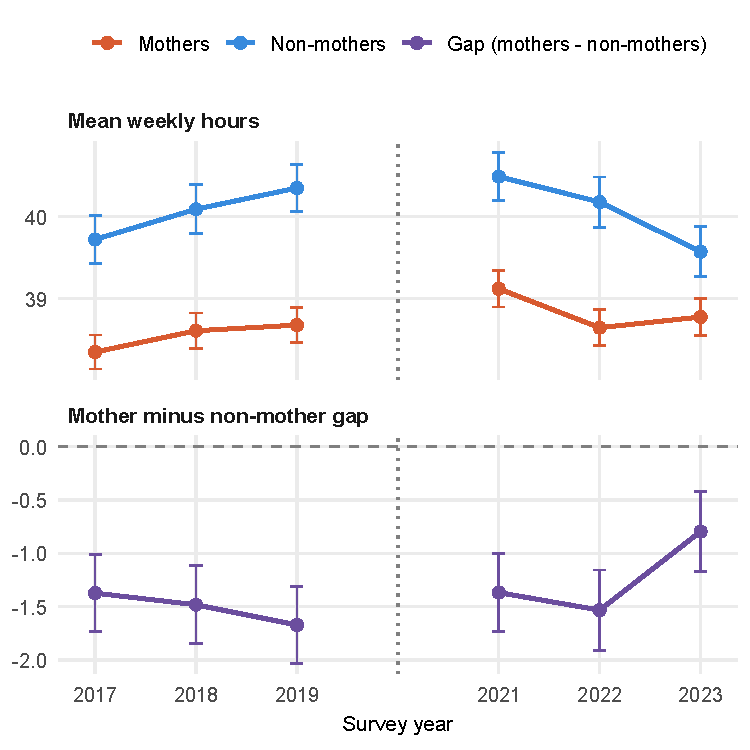
\includegraphics[width=0.7\textwidth]{../outputs/figures/hours_by_year.pdf}
\caption{Weekly hours by survey year: levels and the motherhood gap}\label{fig:hours-by-year}
\begin{minipage}{0.8\textwidth}\small
\vspace{0.3em}
\emph{Notes:} Women aged 25--59 who worked in the reference week, unweighted means with no
controls. The upper panel plots each group's mean weekly hours; the lower panel plots their
difference. Vertical bars are 95\% confidence intervals clustered by individual. The dotted rule
marks the excluded 2020 survey year, and the series break there rather than interpolating across
it. The three pre-period gaps are the raw counterpart of the insignificant $\Mother \times$ year
coefficients in Figure~\ref{fig:pretrend}.
\end{minipage}
\end{figure}

\subsection{Exposure and the commuting channel}\label{sec:desc-exposure}

The triple difference asks whether hours respond where work can be done from home.
Figure~\ref{fig:dose-response} puts that question to the data directly, by computing the same
difference-in-differences as Section~\ref{sec:desc-hours} separately within each quartile of
occupational WFH exposure. The answer is not that the response is larger at the top; it is that
there is no response anywhere else. The bottom three quartiles return $-0.32$, $0.27$ and $-0.02$
hours, none of them distinguishable from zero. The top quartile returns $1.55$ hours
(95\% CI $[0.74, 2.36]$).

Two things follow. First, this is why Section~\ref{sec:desc-hours}'s average is near zero: it is a
weighted average of three nulls and one substantial positive difference, and the three nulls
dominate by construction. The decomposition is approximate rather than exact --- these quartiles
additionally require a matched occupation code, so they rest on $251{,}968$ rows against
Section~\ref{sec:desc-hours}'s $258{,}175$, and the quartile-weighted average is $0.29$ rather than
$0.27$. Second, the dose-response that the DDD coefficient of $3.224$ summarises as a single slope
is visible without any regression --- but it is emphatically not linear in exposure, and the
identifying contrast is a comparison of the most teleworkable quartile against the rest rather than
a smooth gradient. The quartile boundaries make the same point: the bottom three quartiles span
exposure values of $0.00$ to $0.30$, while the top quartile spans $0.30$ to $0.75$. Most of the
dispersion in the regressor lives in one tail, which is worth bearing in mind when reading a
coefficient expressed per unit of exposure.

\begin{figure}[htbp]
\centering
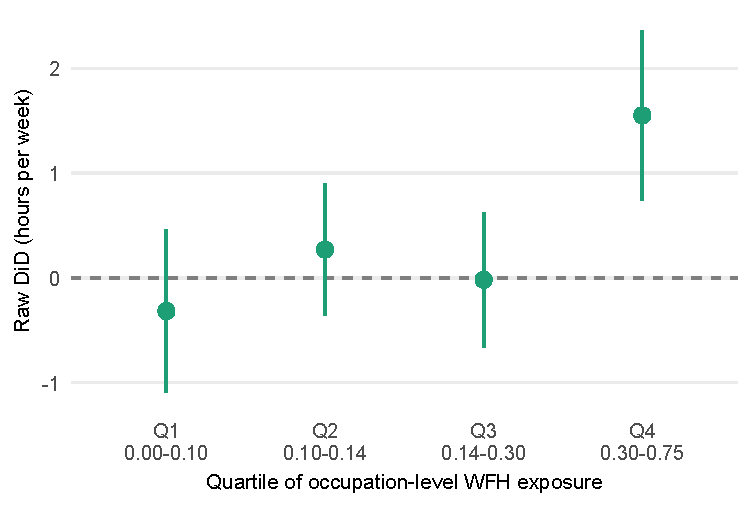
\includegraphics[width=0.8\textwidth]{../outputs/figures/hours_dose_response.pdf}
\caption{Raw hours difference-in-differences by quartile of WFH exposure}\label{fig:dose-response}
\begin{minipage}{0.8\textwidth}\small
\vspace{0.3em}
\emph{Notes:} Women aged 25--59 who worked in the reference week and carry a matched occupation
code. Each point is the
$(\text{mothers post} - \text{mothers pre}) - (\text{childless post} - \text{childless pre})$
difference within one exposure quartile, from unweighted cell means with no controls; bars are 95\%
confidence intervals clustered by individual. Quartiles are of the \emph{occupation-level
calibrated} exposure measure, the same regressor the hours DDD uses. Breakpoints are computed on
pre-period rows and applied to all years, and each quartile's exposure range is printed beneath
its tick: the bottom three quartiles together span exposure $0.00$ to $0.30$ while the top spans
$0.30$ to $0.75$.
\end{minipage}
\end{figure}

Commuting patterns are consistent with this channel. Among women aged 25--59 with a recorded
locality of work, mothers were the \emph{more} mobile group in every year --- working outside their
locality of residence $48.2\%$ of the time in 2019 against $46.1\%$ of childless women --- and
their commuting was the less disturbed by the pandemic: the share fell $1.5$ percentage points for
mothers in 2021 against $3.9$ for childless women, a difference of $2.39$ points (SE $1.17$), with
both series back at their 2019 levels by 2023. That fits a mechanism in which remote work relaxes a
time constraint for women who were already commuting rather than drawing a previously home-bound
group into work. It is descriptive evidence on the mechanism rather than a test of it; no
specification in this paper uses locality of work as an outcome.

%======================================================================
\section{Empirical Strategy}\label{sec:strategy}
%======================================================================

\subsection{Hypothesis}

The flexibility framework of \citet{goldin2014}, as set out in Section~\ref{sec:lit}, yields one
testable hypothesis. \textbf{H1:} after 2021, mothers' usual hours conditional on working rise
relative to childless women's in proportion to their occupation's WFH exposure, with no response
where the work cannot be done from home. The average change in mothers' hours is not the object of
interest; the exposure gradient is. We also estimate the employment margin for completeness
(Section~\ref{sec:res-extensive}).

\subsection{Difference-in-differences}

For outcome $Y_{it}$ (weekly hours conditional on working that week, or employment) we estimate
\begin{equation}\label{eq:did}
Y_{it} = \beta_0 + \beta_1 \Mother_i + \beta_2 \Post_t + \beta_3 (\Mother_i \times \Post_t)
+ X'_{it}\gamma + \varepsilon_{it},
\end{equation}
where $X_{it}$ is the control vector described above. $\beta_3$ is the DiD estimator: the
differential change in the outcome for mothers relative to childless women after the shift to
remote work. For hours, a positive $\beta_3$ indicates a narrowing of the penalty on the intensive
margin.

\subsection{Triple differences}

To test whether the narrowing operates through remote work, we interact the DiD with occupational
WFH exposure:
\begin{equation}\label{eq:ddd}
\begin{split}
Y_{it} = {}& \alpha + \delta_1 \Mother_i + \delta_2 \Post_t + \delta_3 \WFH_{j(i)}
+ \delta_4 (\Mother_i \times \Post_t) \\
& + \delta_5 (\Mother_i \times \WFH_{j(i)}) + \delta_6 (\Post_t \times \WFH_{j(i)}) \\
& + \delta_7 (\Mother_i \times \Post_t \times \WFH_{j(i)}) + X'_{it}\gamma + \varepsilon_{it},
\end{split}
\end{equation}
where $j(i)$ is individual $i$'s occupation. The coefficient of interest, $\delta_7$, asks whether
the post-shift change for mothers relative to non-mothers is larger in more exposed occupations.
The lower-order terms do specific work. $\delta_6$ absorbs any post-2021 change in hours in
teleworkable occupations that is common to mothers and childless women alike --- the general
remote-work recovery --- so that $\delta_7$ is not contaminated by it. $\delta_5$ absorbs the
pre-existing level of the motherhood penalty across occupations, so that $\delta_7$ is a change
and not a level. And $\delta_4$ is the post-shift change for mothers at \emph{zero} exposure, not
an average effect. Following \citet{olden2022}, the DDD does not require two parallel-trends
assumptions but a single one: that the mother/non-mother gap in high- versus low-exposure jobs
would have evolved in parallel absent the shift to remote work.

For the hours DDD, $\WFH_j$ is the calibrated occupation-level score of
Section~\ref{sec:exposure} and the sample is employed women matched to a two-digit occupation. For
the employment DDD, $\WFH$ is the cell-based shift-share index, the sample is all women, employed
or not, and a $\Mother \times$ age-group interaction is added to correct a documented pre-period
age imbalance between mothers and non-mothers.

Equation~\eqref{eq:ddd} makes each lower-order occupation-level difference linear in exposure.
With only forty occupations that restriction is unnecessary, so we estimate two relaxations of it
alongside the pooled model. The \emph{saturated} specification replaces every lower-order term
with fixed effects,
\begin{equation}\label{eq:ddd-sat}
Y_{it} = \delta_7 (\Mother_i \times \Post_t \times \WFH_{j(i)}) + X'_{it}\gamma
+ \lambda_{j(i),t} + \mu_{j(i),\Mother_i} + \nu_{\Mother_i,t} + \varepsilon_{it},
\end{equation}
where $\lambda_{jt}$ are occupation-by-survey-year effects (absorbing $\delta_2$, $\delta_3$,
$\delta_6$ and any occupation-specific year shock), $\mu_{j,m}$ are occupation-by-mother effects
(absorbing $\delta_1$ and $\delta_5$), and $\nu_{m,t}$ are mother-by-year effects (absorbing
$\delta_4$). Only the triple interaction carries a functional form. The \emph{binned}
specification keeps the pooled model's structure but replaces $\WFH_{j(i)}$ with indicators for
the quartile of exposure the occupation falls in --- the same pre-period quartiles as the
dose-response figure of Section~\ref{sec:desc-exposure} --- so that the top-versus-bottom
contrast is reported as a coefficient with a standard error rather than read off a figure. For each DDD we also report the minimum detectable
effect, $\mathrm{MDE} = \mathrm{SE} \times (z_{0.975} + z_{0.80}) = 2.8016 \times \mathrm{SE}$, so
that a null coefficient can be read as ``genuinely null'' or ``underpowered.''

\subsection{Inference}\label{sec:inference}

The survey is a rotating panel: the hours estimation sample of $258{,}175$ observations comes from
only $64{,}602$ distinct respondents --- about four observations each, and two to three within a
single survey year, with $96\%$ of rows belonging to someone who appears more than once. Treating
those observations as independent would understate standard errors by a factor of roughly $1.8$,
so equation~\eqref{eq:did} and every descriptive interval in Section~\ref{sec:descriptives} are
clustered by individual. What the panel structure does \emph{not} support is within-person
identification: only 1.9\% of respondents are re-interviewed across the pre/post boundary, so an
individual fixed-effects design was considered and rejected.
% Provenance: 1,514 of 80,560 distinct individuals (1.88%) appear in both the pre- and post-period.
% Console output of check_idpuf_panel_structure() (scripts/validation.R); not exported to outputs/.
% Confirmed against a full pipeline run, 2026-09-19.

For the hours DDD the regressor of interest is constant within a two-digit occupation, and standard
errors are clustered at that level --- individual-level clustering would understate them. That
leaves forty clusters. The reported $p$-values use \texttt{fixest}'s default small-sample
convention, a $t$ reference distribution with $G - 1 = 39$ degrees of freedom and a cluster-count
adjustment to the variance. Forty is few enough that we do not rest on that approximation. For
the headline coefficient and for the pre-period coefficients of the triple-difference event study
we also report wild cluster bootstrap $p$-values, with Rademacher weights, the null imposed and
$9{,}999$ draws \citep{roodman2019}, computed with the \texttt{fwildclusterboot} package
\citep{fischer2021}. The \emph{joint} pre-period test remains the analytic Wald $F$: the joint
bootstrap is not available in that implementation without a Julia toolchain, so we report the
bootstrap for each pre-period coefficient and for their sum instead. Section~\ref{sec:diagnostics}
adds a permutation test that relies on no asymptotic approximation at all. Clustering two ways, by
individual and by occupation, leaves the headline standard error unchanged
(Section~\ref{sec:res-robust}). The employment DDD is clustered on the age-by-education-by-district
cell (about 210 clusters).

\subsection{Selection into employment: Lee bounds}\label{sec:lee}

Hours are observed only for women who are working, and whether a woman is working is itself an
outcome of the same treatment. If remote work differentially pulls marginal mothers into work after
2021, the post-period sample of working mothers is compositionally different from the pre-period one
for reasons unrelated to hours choices, biasing $\beta_3$ in the hours equation in a direction that
is not signable a priori. We address this with trimming bounds in the spirit of \citet{lee2009},
adapted to the two-by-two design. Let $s_{ab} = \Pr(\text{hours observed} \mid \Mother=a, \Post=b)$
--- that is, the probability of being employed \emph{and} working in the reference week, which is
the sample the outcome is measured on rather than the employed population as a whole.
The counterfactual below assumes parallel trends \emph{in selection}. For post-period mothers it is
$s^*_{11} = s_{10} + (s_{01} - s_{00})$. If the observed $s_{11}$ exceeds $s^*_{11}$, the excess
share $p = 1 - s^*_{11}/s_{11}$ is trimmed from the $(\Mother=1,\Post=1)$ cell's hours
distribution --- from the top to obtain a lower bound on $\beta_3$, from the bottom to obtain an
upper bound --- and equation~\eqref{eq:did} is re-estimated on each trimmed sample. Trimming from a
single tail assumes monotone selection: that remote work weakly increases, and never decreases, a
mother's probability of being observed with hours.

For the DDD we generalize this construction. The selection counterfactual is computed separately
within each quartile of the cell-based exposure index (which, unlike the occupation-level index, is
observable for the non-employed), each quartile's post-period mothers are trimmed by that
quartile's own excess share, the trimmed subsets are recombined, and equation~\eqref{eq:ddd} is
refit with the occupation-level regressor. This stratification assumes that selection into
observed hours depends on exposure only through the cell-index quartile; it is an approximation,
since the outcome equation uses the occupation-level index, and the bound is valid to the extent
that assumption holds. Because the parameter is only partially identified, we report, alongside
each bound's own cluster-robust confidence interval, the \citet{imbens2004} confidence interval for
the identified set, which accounts jointly for the sampling uncertainty of both endpoints. The
construction handles only \emph{excess} selection in the treated cell
(Section~\ref{sec:limitations}).

\subsection{Diagnostics, falsification, and the fathers' comparison}\label{sec:diagnostics}

We estimate event-study versions of equation~\eqref{eq:did} with $\Mother \times$ year
interactions (reference year 2019) for both outcomes and test the pre-period coefficients jointly.
Because those test the difference-in-differences assumption rather than the triple-differences one,
we also estimate the event-study version of equation~\eqref{eq:ddd} itself --- $\Post$ replaced by
survey-year interactions at every level, so that $\Mother \times$ year $\times \WFH$ is recovered
separately for each year --- and apply the same joint test to its pre-period coefficients.

The falsification test is a permutation test on the exposure score. Under the sharp null that
teleworkability is unrelated to the post-2021 change in the motherhood gap, the forty occupation
scores are exchangeable across occupations. We therefore reassign the forty scores at random
across the forty occupation codes $999$ times, holding every woman's occupation and the
mother/period structure fixed, refit equation~\eqref{eq:ddd} each time, and record the
cluster-robust $t$-statistic of the triple interaction. The permutation $p$-value is the share of
draws, counting the observed one, whose $|t|$ reaches the observed value \citep{phipson2010}.
Because it is built from the design itself, it needs neither the $t(39)$ approximation nor a
bootstrap, and it answers the question a placebo should: how often would a design like this one
produce an exposure gradient as large as ours when exposure is, by construction, noise.

The remaining checks re-estimate the hours DDD with an added $\Mother \times$ age-group
interaction and with pre-period age-group raking weights, in response to the age imbalance noted
above; with the external and realized exposure indices in place of the calibrated one; with
alternative codings of the hours outcome; separately for Jewish and Arab women; by the age of the
youngest child; and on the male subsample with ``mother'' read as ``father.'' The last of these is
a comparison, not a placebo: fathers in teleworkable occupations are exposed to remote work exactly
as mothers are, so a null for fathers is not what the design predicts, and a negative gradient
would be evidence on household reallocation rather than on a confound. Coefficients across
subsamples are compared with two-sample $z$-tests, which are valid without a covariance
correction because the samples are disjoint.

%======================================================================
\section{Results}\label{sec:results}
%======================================================================

Throughout, significance is denoted \sym{***} $p<0.001$, \sym{**} $p<0.01$, \sym{*} $p<0.05$,
\sym{\cdot} $p<0.1$. Standard errors are in parentheses.

\subsection{Pre-trends and the hours DiD}\label{sec:res-did}

Before turning to the estimates, Figure~\ref{fig:pretrend} reports the hours event study. Relative
to 2019, neither pre-period $\Mother \times$ year coefficient is distinguishable from zero ---
$0.3515$ in 2017 and $0.2013$ in 2018 --- and a joint Wald test on the two does not reject
($F(2, 63{,}198) = 0.949$, $p = 0.387$). The same test on the employment outcome also passes
(Section~\ref{sec:res-extensive}), so the difference-in-differences identifying assumption is
supported on both margins over the full pre-period. The triple difference rests on a different and
stricter assumption, which requires an event study of its own (Section~\ref{sec:res-ddd-diag}). In
the post-period the effect builds gradually --- $0.3923$ in 2021, $0.1213$ in 2022, and
$0.7517$\sym{**} in 2023 --- and Figure~\ref{fig:hours-by-year} shows the corresponding raw gaps
with no regression adjustment at all.

\begin{figure}[htbp]
\centering
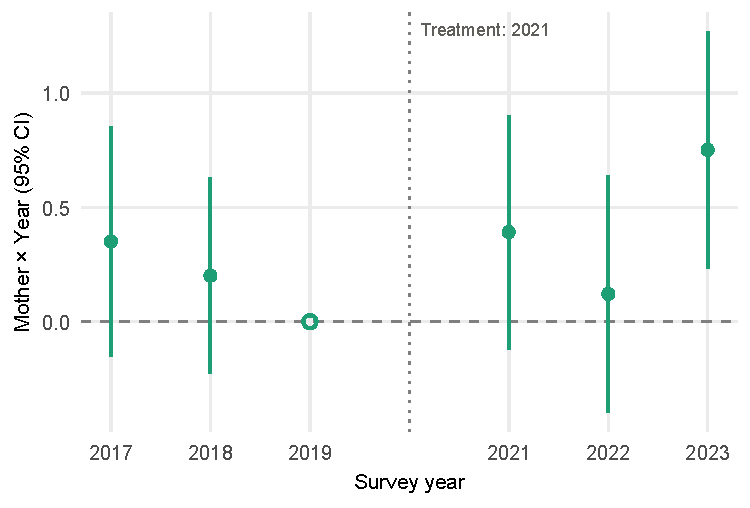
\includegraphics[width=0.7\textwidth]{../outputs/figures/hours_event_study.pdf}
\caption{Event study: $\Mother \times$ year interactions for weekly hours, reference year
2019}\label{fig:pretrend}
\begin{minipage}{0.8\textwidth}\small
\vspace{0.3em}
\emph{Notes:} Women working in the reference week ($N = 251{,}857$); standard controls; standard
errors clustered by individual. Vertical bars are 95\% confidence intervals. Coefficients (SE):
2017, $0.3515$ ($0.2570$); 2018, $0.2013$ ($0.2191$); 2021, $0.3923$ ($0.2612$); 2022, $0.1213$
($0.2654$); 2023, $0.7517$\sym{**} ($0.2650$). Joint test on 2017--2018: $F(2, 63{,}198) = 0.949$,
$p = 0.387$. The hollow point at 2019 is the omitted reference year, pinned at zero by construction
rather than estimated. The gap between 2019 and 2021 is the excluded 2020 survey year; the dotted
rule marks the treatment boundary.
\end{minipage}
\end{figure}

Column~(1) of Table~\ref{tab:hours} reports equation~\eqref{eq:did} for weekly hours among women
working in the reference week. Mothers work $1.739$ fewer hours per week than childless women
($\Mother = -1.739$\sym{***}), the intensive-margin penalty itself. That penalty did not
measurably change after the shift to remote work: $\Mother \times \Post = 0.2280$ (SE $0.1809$),
$t = 1.26$, $N = 251{,}857$. The raw cell means of Section~\ref{sec:desc-hours} agree on magnitude:
the unadjusted difference-in-differences is $0.266$, so the controls move the estimate by less than
four hundredths of an hour. They do not agree on precision --- the unclustered standard error is
$0.098$, roughly half the clustered one --- which is why the raw arithmetic should not be read as
evidence of a significant increase. At this standard error the minimum detectable effect is
$2.8016 \times 0.1809 \approx 0.51$ hours, so the estimate rules out average gains much above half
an hour a week: a reasonably precise null, not an uninformative one. Replacing the single
$\Post$ dummy with survey-year effects, so that the year-to-year movements of
Figure~\ref{fig:hours-by-year} are absorbed rather than pooled, leaves it at $0.2310$
(SE $0.1808$).

Selection into the estimation sample does not change that reading. The probability that hours are
observed for post-period mothers ($s_{11} = 0.6964$) exceeds the parallel-trends-in-selection
counterfactual ($s^*_{11} = 0.6786 + (0.7058 - 0.7010) = 0.6833$), so there is excess selection to
trim --- about 1.9\% of the cell.\footnote{Derived as $1 - 0.6833/0.6964$ from the selection rates
$s_{00} = 0.7010$, $s_{01} = 0.7058$, $s_{10} = 0.6786$ and $s_{11} = 0.6964$; not directly exported
by the pipeline.} The resulting Lee bounds are $-0.5166$ (SE $0.1781$) and $0.8017$ (SE $0.1789$),
with an Imbens--Manski 95\% confidence interval for the identified set of $[-0.810, 1.096]$. The
correction widens the interval around a null rather than overturning a finding. We therefore do not
treat the plain hours DiD as evidence of an average effect in either direction, and nothing that
follows rests on it.

\subsection{The hours DDD: the paper's headline result}\label{sec:res-ddd}

Column~(2) of Table~\ref{tab:hours} interacts the DiD with the calibrated occupation-level
exposure index. The triple interaction is $3.224$\sym{**} (SE $1.022$, $N = 246{,}326$): among
mothers who are working, those in more WFH-exposed occupations saw a larger post-2021 increase in
weekly hours relative to childless women in the same occupations --- about $3.2$ additional hours
per unit of exposure. A unit is not a movement the data contain, so the coefficient needs a scale.
On the estimation sample the calibrated index has a standard deviation of $0.199$ and an
interquartile range of $0.203$, so the estimate is $0.64$ hours per standard deviation of exposure
and $0.65$ hours per interquartile range. Between the quartiles of Figure~\ref{fig:dose-response},
whose mean exposures are $0.06$ at the bottom and $0.59$ at the top, the regression implies a
difference of $1.71$ hours a week. The raw quartile difference-in-differences of that figure put the
same contrast at $1.87$ hours ($1.55$ against $-0.32$), within a fifth of an hour of the linear
model's implication; that agreement is the paper's one check on the linear-in-exposure functional
form, and it holds even though the regressor's dispersion is concentrated in the top quartile.

The column's second row is as informative as its first. At zero exposure --- an occupation that
cannot be done from home at all --- the implied change for mothers is $\Mother \times \Post =
-0.5385$ (SE $0.3364$), if anything negative. And because $\Post \times \WFH$ is in the model, the
gradient is net of whatever happened to hours in teleworkable occupations for all women. Set against
the near-zero average effect of column~(1), the reading is not that a broad gain is \emph{larger}
in teleworkable jobs. It is that outside teleworkable jobs there is no gain to speak of, and the
entire effect is the exposure gradient. That is a sharper claim than the one a significant average
DiD would have supported, and it is the claim Figure~\ref{fig:dose-response} shows directly: three
quartiles at zero and one well above it.

The estimate is $3.15$ analytic standard errors from zero; Section~\ref{sec:res-robust} reports
the bootstrap and permutation $p$-values that qualify that figure. The design's minimum
detectable effect is $2.864$ hours per unit of exposure, or $0.57$ hours per standard deviation
($7.3\%$ of mean weekly hours), so an effect of the size observed is detectable, though without
a great deal of room to spare; the reweighted specification of Section~\ref{sec:res-robust}
shows what that margin means in practice.

Columns~(3) and~(4) relax the functional form. With occupation-by-year, occupation-by-mother and
mother-by-year fixed effects in place of every lower-order term (equation~\eqref{eq:ddd-sat}),
the triple interaction is $2.876$ (SE $0.9495$), about a tenth below the pooled estimate and
still significant at the $1\%$ level on the analytic standard error: the linear lower-order
terms of column~(2) are not what produces the result. Column~(4) replaces the score with
indicators for the pre-period exposure quartile the occupation falls in, the bins of
Figure~\ref{fig:dose-response}. Relative to the least teleworkable quartile, the post-2021
change in the mother/non-mother gap is $0.75$ hours (SE $0.48$) in the second quartile, $0.60$
(SE $0.48$) in the third, and $1.844$ (SE $0.594$, $p < 0.01$) in the top quartile. The
top-quartile contrast is the between-quartile difference the linear model implies ($1.71$) and
the raw figure shows ($1.87$), now carrying a standard error, and it is the only quartile
contrast that is individually significant: the response is a step at the top of the exposure
distribution more than a smooth gradient across it. That top quartile holds six of the forty
occupations (sixteen, seven, eleven and six from the bottom up), which is why it matters that
the pooled and saturated columns, which use all forty, agree with it in sign and magnitude.

\begin{table}[htbp]
\centering
\begin{threeparttable}
\caption{Intensive-margin DiD and DDD: weekly hours, reference-week workers}\label{tab:hours}
\renewcommand{\baselinestretch}{1}\scriptsize
\setlength{\tabcolsep}{3pt}
\begin{tabular}{lcccc}
\toprule
 & (1) DiD & (2) DDD & (3) DDD, saturated & (4) DDD, quartiles \\
\midrule
Mother $\times$ Post $\times$ WFH\_Exposure &  & $3.224$\sym{**} & $2.876$\sym{**} &  \\
 &  & $(1.022)$ & $(0.9495)$ &  \\
Mother $\times$ Post $\times$ Q2 (vs.\ Q1) &  &  &  & $0.7529$ \\
 &  &  &  & $(0.4827)$ \\
Mother $\times$ Post $\times$ Q3 (vs.\ Q1) &  &  &  & $0.5998$ \\
 &  &  &  & $(0.4847)$ \\
Mother $\times$ Post $\times$ Q4 (vs.\ Q1) &  &  &  & $1.844$\sym{**} \\
 &  &  &  & $(0.5946)$ \\
Mother $\times$ Post & $0.2280$ & $-0.5385$ &  & $-0.4720$ \\
 & $(0.1809)$ & $(0.3364)$ &  & $(0.3459)$ \\
Mother $\times$ WFH\_Exposure &  & $-1.295$ &  &  \\
 &  & $(1.053)$ &  &  \\
Post $\times$ WFH\_Exposure &  & $-0.5483$ &  &  \\
 &  & $(0.8102)$ &  &  \\
WFH\_Exposure &  & $1.128$ &  &  \\
 &  & $(3.912)$ &  &  \\
Mother & $-1.739$\sym{***} & $-1.449$\sym{***} &  & $-1.527$\sym{**} \\
 & $(0.1441)$ & $(0.3512)$ &  & $(0.4523)$ \\
Post & $-0.0570$ & $0.0535$ &  & $-0.1305$ \\
 & $(0.1481)$ & $(0.2732)$ &  & $(0.3666)$ \\
Constant & $32.35$\sym{***} & $32.12$\sym{***} &  & $31.58$\sym{***} \\
 & $(0.3182)$ & $(1.540)$ &  & $(2.051)$ \\
\midrule
MDE for triple interaction &  & $2.8640$ &  &  \\
SD of exposure, estimation sample &  & $0.1986$ &  &  \\
Triple interaction per SD of exposure &  & $0.640$ &  &  \\
Occupations in Q1 / Q2 / Q3 / Q4 &  &  &  & 16 / 7 / 11 / 6 \\
Fixed effects & None & None & Three sets & None \\
Observations & 251{,}857 & 246{,}326 & 246{,}324 & 246{,}326 \\
$R^2$ & 0.04049 & 0.04094 & 0.13512 & 0.04815 \\
Clustering & individual & occupation (40) & occupation (40) & occupation (40) \\
\bottomrule
\end{tabular}

\begin{tablenotes}\small
\item Dependent variable: usual weekly work hours, women working in the reference week. Standard
controls in every column. Columns (2)--(4) use the calibrated occupation-level exposure index
on column (1)'s sample less the rows with no matched 2-digit occupation. Column (3) is
equation~\eqref{eq:ddd-sat}: the ``three sets'' of fixed effects are occupation $\times$ year,
occupation $\times$ mother and mother $\times$ year, which absorb every lower-order term, so
only the triple interaction is reported. Column (4) replaces the score with indicators for its pre-period quartile
(Figure~\ref{fig:dose-response}'s bins) and reports the three quartile contrasts against the
bottom quartile; its lower-order quartile terms are estimated but not shown, and the number of
occupations in each bin is listed because occupation is the cluster. MDE at $\alpha = 0.05$,
power $0.80$. Columns (2)--(4) use a $t$ reference distribution with 39 degrees of freedom
(Section~\ref{sec:inference}); the wild-bootstrap and permutation $p$-values for column (2)'s
triple interaction are in Table~\ref{tab:robust}. Column (2)'s $\Mother \times \Post$ is the
effect at \emph{zero} exposure, not an average effect. \autonoteHours
\end{tablenotes}
\end{threeparttable}
\end{table}

\subsection{Diagnostics for the triple difference}\label{sec:res-ddd-diag}

\paragraph{Pre-trends.}
The pre-trend test of Figure~\ref{fig:pretrend} licenses equation~\eqref{eq:did}, not
equation~\eqref{eq:ddd}. It asks whether mothers and childless women trended together; the triple
difference requires the stricter condition that the mother/non-mother gap trended together
\emph{across levels of WFH exposure}. These are not the same assumption, and the
difference-in-differences version is not the conservative one: because it averages over exposure, a
pre-period divergence correlated with exposure but netting to zero across occupations would leave
the DiD test untouched while invalidating the headline estimate. Figure~\ref{fig:pretrend-ddd}
therefore reports the event-study analogue of equation~\eqref{eq:ddd}, on the same sample,
exposure index and clustering as column~(2) of Table~\ref{tab:hours}.

The result is supportive. Neither pre-period coefficient is close to significant, and neither is
far from zero in level: $0.5866$ in 2017 and $0.3134$ in 2018, against post-period estimates five to
thirteen times larger. The joint Wald test does not reject, and does not come near rejecting
($F(2, 39) = 0.041$, $p = 0.960$). The post-period path is flat, then steps up in 2021 and rises:
$3.011$\sym{*}, $3.545$\sym{**}, $4.020$\sym{**}, all three individually significant and straddling
the pooled $3.224$ of Table~\ref{tab:hours}, which is what a treatment beginning in 2021 looks like
rather than a pre-existing trend carried through the sample.

One caveat belongs with this test rather than in a footnote. Clustering at the level the exposure
regressor actually varies at leaves forty occupation clusters, so the pre-period standard errors
($2.2367$ and $1.7449$) are of the same order as the effect being tested. Each pre-period confidence
interval therefore contains values larger in magnitude than $3.224$: the test is consistent with
parallel trends and shows no sign of a violation, but it does not have the power to rule out a
pre-trend as large as the estimate itself. The wild cluster bootstrap does not change that
reading: the bootstrap $p$-values are $0.84$ for the 2017 coefficient, $0.88$ for 2018 and
$0.85$ for their sum. This is the same small-cluster limitation the headline estimate carries,
and we read it as supporting evidence rather than as a closed question.

\begin{figure}[htbp]
\centering
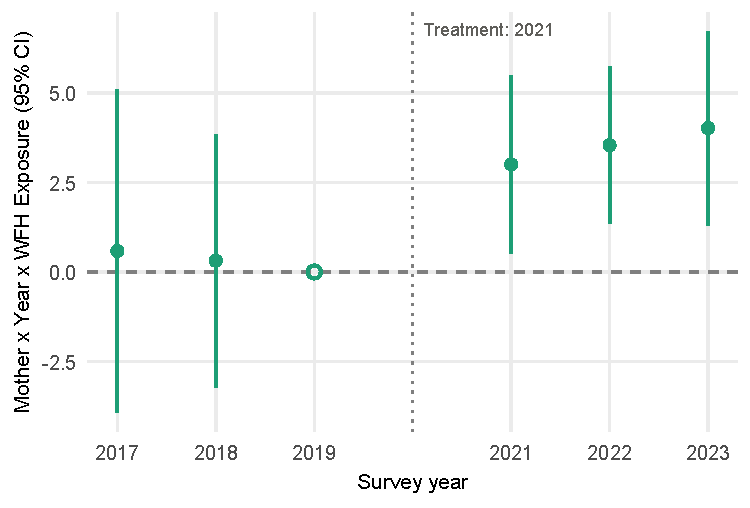
\includegraphics[width=0.7\textwidth]{../outputs/figures/hours_ddd_event_study.pdf}
\caption{Event study for the triple difference: $\Mother \times$ year $\times$ $\WFH$ interactions
for weekly hours, reference year 2019}\label{fig:pretrend-ddd}
\begin{minipage}{0.8\textwidth}\small
\vspace{0.3em}
\emph{Notes:} Employed women matched to a two-digit occupation and working in the reference week
($N = 246{,}326$); standard controls; calibrated occupation-level exposure; standard errors
clustered by two-digit occupation (40 clusters). Vertical bars are 95\% confidence intervals.
Coefficients (SE), hours per unit of exposure: 2017, $0.5866$ ($2.2367$); 2018, $0.3134$
($1.7449$); 2021, $3.0114$\sym{*} ($1.2327$); 2022, $3.5454$\sym{**} ($1.0850$); 2023,
$4.0203$\sym{**} ($1.3397$). Joint test on 2017--2018: $F(2, 39) = 0.041$, $p = 0.960$; wild
cluster bootstrap $p$-values (Rademacher, $9{,}999$ draws) $0.838$ for 2017, $0.884$ for 2018 and
$0.852$ for their sum. The
specification includes the year main effects and both two-way year interactions ($\Mother \times$
year and $\WFH \times$ year) alongside the triple interaction plotted here; omitting any of them
would make the estimate a two-way difference rather than a triple one. The hollow point at 2019 is
the omitted reference year. The gap between 2019 and 2021 is the excluded 2020 survey year; the
dotted rule marks the treatment boundary. Compare Figure~\ref{fig:pretrend}, which plots the
difference-in-differences analogue and tests a weaker assumption.
\end{minipage}
\end{figure}

\paragraph{Lee bounds.}
Table~\ref{tab:lee-ddd} applies the generalized selection correction. Excess selection into the
estimation sample among post-period mothers is present in all four quartiles of the cell-based
exposure index but modest everywhere: the trim proportion ranges from $0.80\%$ (quartile 3) to
$4.48\%$ (quartile 1, the least teleworkable jobs), and a total of $1{,}396$ of $72{,}820$
post-period working mothers are trimmed. The bounds move little: the lower bound is $3.1255$
(SE $1.1440$), the upper bound $3.4434$ (SE $1.0220$), and the Imbens--Manski 95\% confidence
interval for the identified set is $[1.021, 5.324]$, which excludes zero. The triple interaction
therefore survives the selection correction, and is the strongest single piece of evidence in the
paper.

\begin{table}[htbp]
\centering
\begin{threeparttable}
\caption{Generalized Lee bounds on the hours DDD ($\Mother \times \Post \times \WFH$)}\label{tab:lee-ddd}
\renewcommand{\baselinestretch}{1}\small
\setlength{\tabcolsep}{3pt} % eight columns; the default 6pt overran the text width by ~40pt
\emph{Panel A: selection rates and trimming by cell-exposure quartile}\par\vspace{0.4em}
\begin{tabular}{lccccccc}
\toprule
Quartile & $s_{00}$ & $s_{01}$ & $s_{10}$ & $s_{11}$ & $s^*_{11}$ & $n(\Mother{=}1,\Post{=}1)$ & Trim \\
\midrule
1 & $0.5830$ & $0.5862$ & $0.5497$ & $0.5788$ & $0.5529$ & 21{,}655 & 4.48\% \\
2 & $0.7070$ & $0.7120$ & $0.6856$ & $0.6977$ & $0.6906$ & 28{,}540 & 1.01\% \\
3 & $0.7542$ & $0.7450$ & $0.7554$ & $0.7522$ & $0.7462$ & 34{,}293 & 0.80\% \\
4 & $0.8194$ & $0.8029$ & $0.7352$ & $0.7399$ & $0.7188$ & 21{,}815 & 2.85\% \\
\bottomrule
\end{tabular}

\par\vspace{0.9em}
\emph{Panel B: bounds on the triple interaction}\par\vspace{0.4em}
\begin{tabular}{lccc}
\toprule
Bound & Coefficient & SE & 95\% CI \\
\midrule
Lower & $3.1255$ & $1.1440$ & $[0.8833,\ 5.3677]$ \\
Point (untrimmed) & $3.2319$ & $1.0538$ & $[1.1664,\ 5.2973]$ \\
Upper & $3.4434$ & $1.0220$ & $[1.4404,\ 5.4465]$ \\
\midrule
Imbens--Manski 95\% CI for the identified set &  &  & $[1.021,\ 5.324]$ \\
\bottomrule
\end{tabular}

\begin{tablenotes}\small
\item $s_{ab}$ is the probability that hours are observed --- employed \emph{and} working in the
reference week --- so these rates are lower than the corresponding employment rates. Panel A's $n$
column counts all post-period mothers in the quartile, working or not, because the cell-based
index is defined for the non-employed as well; the trim proportions apply to the occupation-matched
subset with observed hours ($1{,}396$ of $72{,}820$ in total), which is the population the bound
regressions use. The untrimmed point estimate here ($3.2319$) differs slightly from
Table~\ref{tab:hours} ($3.224$) because this sample additionally requires a matched cell-based
exposure. Outcome regressions use the occupation-level index and cluster by occupation.
\end{tablenotes}
\end{threeparttable}
\end{table}

\subsection{Robustness}\label{sec:res-robust}

Table~\ref{tab:robust} collects the remaining checks.

\paragraph{Exposure measure.}
With the raw \citet{dingel2020} external index in place of the calibrated one, the triple
interaction is $0.6720$ (SE $0.8838$), positive but insignificant; with the realized 2021-anchored
index it is $5.195$\sym{*} (SE $2.363$). The direction is consistent across all three measures but
the magnitude and significance are not, and we describe the result as directionally rather than
point-estimate robust to the exposure measure.

That pattern deserves a direct statement, because it is the natural objection to the design. The
external index is the only one of the three built entirely from pre-treatment information, and it
yields the weakest estimate; the two that draw on post-period Israeli data yield significant ones.
One reading, which we hold, is that the mechanism becomes visible only once exposure is measured as
Israeli jobs were actually done rather than as US task content says they could be: teaching and
clerical support, which the external index scores as almost fully teleworkable, returned fully to
the workplace, and an index that places them in the treated tail is measuring the wrong thing.
The other reading is that calibrating on 2022--23 realized WFH lets the regressor absorb
post-period outcomes. Four features of the construction limit that risk: the realized shares are
computed on men and women together, not on the women in the regression; only ten of forty
occupations are swapped, and only where the gap exceeds $0.5$ and a one-sided test at the 95\%
level rejects sampling noise; all ten swaps are \emph{downward}, removing occupations from the
treated tail rather than adding any to it; and the outcome is usual hours, not the WFH indicator
the calibration uses. The direct test is to drop the ten swapped occupations and re-estimate on
the thirty where the calibrated and external indices coincide by construction, so that no
post-period information enters the regressor at all. On that sample the triple interaction is
$4.309$\sym{**} (SE $1.192$, $N = 132{,}046$, 30 clusters), larger than the headline, not
smaller. The post-period calibration does not produce the result; if anything the ten swapped
occupations, which together account for nearly half the estimation sample, dilute it. What the
calibration cannot be made into is a pre-treatment measure.

\paragraph{Age balance.}
Adding a $\Mother \times$ age-group interaction leaves the estimate essentially unchanged
($3.205$\sym{**}, SE $1.055$). Reweighting the sample to balance pre-period age groups between
mothers and non-mothers attenuates it by about 19\% to $2.597$\sym{*} (SE $1.050$) --- still
significant, though at the 5\% level rather than the 1\%, and a value the design would detect only
narrowly (its minimum detectable effect is $2.864$), so we would not rest the result on this
specification alone. The imbalance being corrected is real and tracks exposure: the pre-period
mother/non-mother gap in the age-group code is $-0.974$ in the lowest exposure quartile
($t = -94.0$), $-0.735$ in the second, $-0.169$ in the third, and $+0.057$ in the highest. The
reweighted attenuation is the largest single move any check produces, and it is worth reporting for
that reason.

\paragraph{Sample.}
Excluding the 2023 survey year, whose final quarter includes the start of the October 2023 war
(Section~\ref{sec:limitations}), the triple interaction is $2.979$\sym{*} (SE $1.170$,
$N = 208{,}833$): smaller, since 2023 carries the largest event-study coefficient, but still
significant at the 5\% level, while the plain hours DiD stays a null ($0.0710$, SE $0.1975$).

\paragraph{Outcome coding.}
The hours variable is a bin-median approximation with two irregular-hours codes imputed from
period-specific medians (Section~\ref{sec:data}), and the effect is smaller than one bin width,
so the result should not depend on how the bins are turned into hours. Dropping the two imputed
codes instead of imputing them gives $3.056$\sym{**} (SE $1.059$, $N = 232{,}785$). Because the
bin medians make 35 and 40 hours exact bin edges, the same specification can be estimated as a
linear probability model on bin-crossing outcomes: the probability of usually working at least
35 hours rises by $0.0964$\sym{**} (SE $0.0291$) per unit of exposure for mothers relative to
childless women after 2021, and the probability of working at least 40 hours by
$0.1073$\sym{**} (SE $0.0380$). Per standard deviation of exposure those are $1.9$ and $2.1$
percentage points, against pre-period shares among working mothers of $71\%$ working at least
35 hours and $61\%$ at least 40. The effect is a shift of mothers in teleworkable jobs across the
full-time boundary, which is the reading Section~\ref{sec:data} anticipated.

\paragraph{Inference.}
Clustering two ways, by individual and by occupation, leaves the headline standard error
unchanged at $1.022$: the occupation-level dependence already dominates the individual-level one.
The forty-cluster problem is not addressed by two-way clustering, and the two procedures of
Section~\ref{sec:inference} that do address it disagree with the analytic $p$-value of $0.003$.
The wild cluster bootstrap gives $p = 0.056$, with a bootstrap 95\% confidence set of
$[-0.26, 5.84]$; the permutation test gives $p = 0.032$, with $31$ of $999$ random reassignments
of the forty exposure scores producing a $|t|$ at least as large as the observed $3.15$
(Section~\ref{sec:res-falsification}). The estimate is therefore significant at the $1\%$ level
on the analytic standard error, at the $5\%$ level under the permutation test, and at the
$10\%$ level under the bootstrap, and we report all three rather than choosing among them. The
bootstrap, which re-signs whole-cluster residuals, is the most conservative of the three; the
permutation test holds the design's cluster structure fixed and randomizes only the regressor,
which is the sharper question for a triple difference whose identifying variation is
occupation-level exposure.

\begin{table}[htbp]
\centering
\begin{threeparttable}
\caption{Hours DDD: sensitivity of $\Mother \times \Post \times \WFH$}\label{tab:robust}
\renewcommand{\baselinestretch}{1}\small
\setlength{\tabcolsep}{3pt}
\begin{tabular}{lcccc}
\toprule
Specification & Coefficient & SE & $p$ & $N$ \\
\midrule
\multicolumn{5}{l}{\emph{Exposure measure}} \\
\quad Calibrated (primary) & $3.224$\sym{**} & $1.022$ & $0.0031$ & 246{,}326 \\
\quad External (Dingel--Neiman) & $0.6720$ & $0.8838$ & $0.4517$ & 246{,}326 \\
\quad Realized (2021 anchor) & $5.195$\sym{*} & $2.363$ & $0.0346$ & 246{,}037 \\
\multicolumn{5}{l}{\emph{Age balance}} \\
\quad Age-interacted ($+\,\Mother \times$ age group) & $3.205$\sym{**} & $1.055$ & $0.0042$ & 246{,}326 \\
\quad Reweighted (pre-period age-group raking) & $2.597$\sym{*} & $1.050$ & $0.0178$ & 242{,}552 \\
\multicolumn{5}{l}{\emph{Sample}} \\
\quad Unswapped occupations only (30 of 40) & $4.309$\sym{**} & $1.192$ & $0.0011$ & 132{,}046 \\
\quad Excluding survey year 2023 & $2.979$\sym{*} & $1.170$ & $0.0151$ & 208{,}833 \\
\multicolumn{5}{l}{\emph{Outcome coding}} \\
\quad Irregular-hours codes dropped, not imputed & $3.056$\sym{**} & $1.059$ & $0.0064$ & 232{,}785 \\
\quad Full-time indicator ($\geq 35$ hours) & $0.0964$\sym{**} & $0.0291$ & $0.0020$ & 246{,}326 \\
\quad Long-hours indicator ($\geq 40$ hours) & $0.1073$\sym{**} & $0.0380$ & $0.0075$ & 246{,}326 \\
\multicolumn{5}{l}{\emph{Inference on the primary estimate}} \\
\quad Two-way clustering (individual, occupation) & $3.224$\sym{**} & $1.022$ & $0.0031$ & 246{,}326 \\
\quad Wild cluster bootstrap ($B = 9{,}999$) & $3.224$ & $1.022$ & $0.0558$ & 246{,}326 \\
\quad Permutation test (999 reassignments) & $3.224$ &  & $0.0320$ & 246{,}326 \\
\bottomrule
\end{tabular}

\begin{tablenotes}\small
\item All rows: the triple interaction $\Mother \times \Post \times \WFH$ from
equation~\eqref{eq:ddd}, women working in the reference week, standard controls, calibrated
exposure unless stated, clustered by occupation unless stated; $p$ is the analytic $t(39)$
$p$-value unless the row says otherwise. The unswapped-occupations row drops the ten occupations
whose exposure was swapped to its realized 2022--23 value, so the calibrated and external indices
coincide on the rows that remain. The two indicator outcomes are linear probability models on
bin-crossing outcomes: the bin medians make 35 and 40 hours exact bin edges. The
no-imputation row drops the two irregular-hours codes instead of imputing them. The
wild-bootstrap row reports the analytic coefficient and standard error with the bootstrap
$p$-value (Section~\ref{sec:inference}); the permutation row reports the permutation $p$-value
of Section~\ref{sec:diagnostics}, which has no standard error.
\end{tablenotes}
\end{threeparttable}
\end{table}

\subsection{Falsification: permuting exposure across occupations}\label{sec:res-falsification}

Figure~\ref{fig:permutation} plots the reference distribution the permutation test builds. Each
of the $999$ draws reassigns the forty calibrated scores at random across the forty occupation
codes, leaving every woman's occupation, her mother status and the survey year untouched, and
refits equation~\eqref{eq:ddd} with occupation-clustered standard errors. Under this sharp null
the design produces cluster-robust $t$-statistics whose central $95\%$ lie between $-2.96$ and
$2.60$, with the largest $|t|$ of any draw at $6.21$; the observed $3.15$ is exceeded in absolute
value by $31$ draws, so $p = 0.032$ (Monte-Carlo standard error $0.006$). Read the other way, a
design with this cluster structure produces an exposure gradient as large as ours about three
times in a hundred when exposure carries no information. That is the falsification a placebo
should supply and a fathers' regression cannot: the latter compares a different, also-treated
population, whereas this test asks the design itself how often it finds a gradient in noise.

\begin{figure}[htbp]
\centering
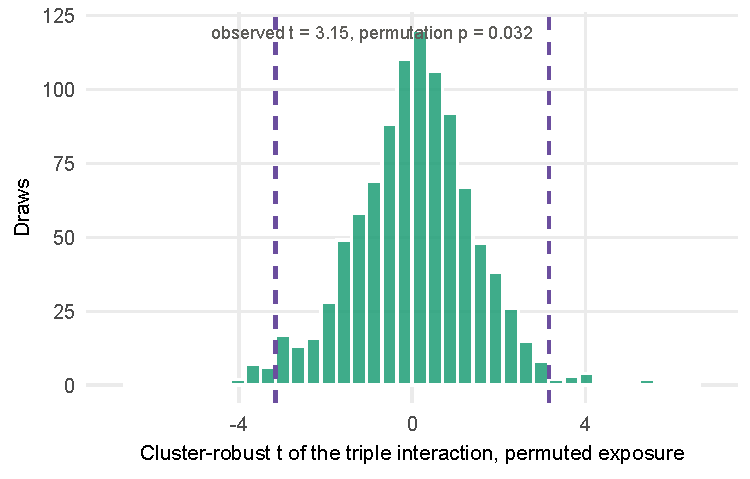
\includegraphics[width=0.75\textwidth]{../outputs/figures/hours_permutation.pdf}
\caption{Permutation distribution of the hours DDD triple interaction}\label{fig:permutation}
\begin{minipage}{0.8\textwidth}\small
\vspace{0.3em}
\emph{Notes:} Histogram of the cluster-robust $t$-statistic of $\Mother \times \Post \times \WFH$
over $999$ random reassignments of the forty occupation-level exposure scores across occupations
(seed fixed in the replication code), with the same sample, controls and clustering as column~(2)
of Table~\ref{tab:hours}. Dashed lines mark $\pm$ the observed statistic ($3.15$); $p = 0.032$
counts the observed draw \citep{phipson2010}.
\end{minipage}
\end{figure}

\subsection{Heterogeneity by the age of the youngest child}\label{sec:res-childage}

If remote work relaxes a time constraint that binds through child care, the response should be
largest for mothers of young children and smallest for mothers whose youngest child is a
teenager. The survey records the youngest child's age in bins, so Table~\ref{tab:childage} and
Figure~\ref{fig:childage} re-estimate the hours DiD and DDD four times, each time comparing one
group of mothers --- those whose youngest child is aged 0--4, 5--9, 10--14 or 15--17 --- with the
same $133{,}646$ childless women. The average effect is a null in every group: the DiD is
between $0.13$ and $0.56$ hours and never distinguishable from zero. The exposure gradient
declines monotonically with the child's age: $3.656$\sym{**} hours per unit of exposure
(SE $1.079$) for mothers of under-fives, $3.211$\sym{*} (SE $1.311$) for youngest children aged
5--9, $2.741$ (SE $1.525$, $p = 0.08$) for 10--14, and $1.862$ (SE $0.935$, $p = 0.05$) for
15--17, half the under-five estimate. Because the four regressions share the control group they
are not independent samples and the two-sample $z$-test of Section~\ref{sec:diagnostics} does
not apply across rows; the individual confidence intervals overlap, so the pattern is a gradient
consistent with the mechanism rather than a set of statistically separated effects. It also
answers the concern that ``mother'' is a broad category: the estimate is not carried by mothers
of teenagers, for whom the time constraint is weakest, and it is largest exactly where the
mechanism predicts.

\begin{table}[htbp]
\centering
\begin{threeparttable}
\caption{Hours DiD and DDD by age of the youngest child}\label{tab:childage}
\renewcommand{\baselinestretch}{1}\small
\setlength{\tabcolsep}{3pt}
\begin{tabular}{lcccccc}
\toprule
 & \multicolumn{3}{c}{DiD: $\Mother \times \Post$} & \multicolumn{3}{c}{DDD: $\Mother \times \Post \times \WFH$} \\
\cmidrule(lr){2-4}\cmidrule(lr){5-7}
Sample of mothers & Coef. & SE & $N$ & Coef. & SE & $N$ \\
\midrule
All mothers (Table~\ref{tab:hours}) & $0.2280$ & $0.1809$ & 251{,}857 & $3.224$\sym{**} & $1.022$ & 246{,}326 \\
\midrule
Youngest child aged 0--4 & $0.1267$ & $0.2111$ & 158{,}424 & $3.656$\sym{**} & $1.079$ & 154{,}499 \\
Youngest child aged 5--9 & $0.1621$ & $0.2533$ & 130{,}782 & $3.211$\sym{*} & $1.311$ & 127{,}419 \\
Youngest child aged 10--14 & $0.1593$ & $0.2780$ & 123{,}280 & $2.741$\sym{\cdot} & $1.525$ & 120{,}084 \\
Youngest child aged 15--17 & $0.5613$ & $0.3483$ & 107{,}061 & $1.862$\sym{\cdot} & $0.9354$ & 104{,}079 \\
\bottomrule
\end{tabular}

\begin{tablenotes}\small
\item Weekly hours, reference-week workers, standard controls; each row compares the named group
of mothers (youngest child's age from the CBS bin variable) with all childless women, so the
control group is identical across rows and the rows are not independent samples. DiD clustered
by individual; DDD clustered by occupation, calibrated exposure. The first row repeats
Table~\ref{tab:hours}. Mothers whose youngest-child code falls outside the four bins enter no
row. \autonoteChildAge
\end{tablenotes}
\end{threeparttable}
\end{table}

\begin{figure}[htbp]
\centering
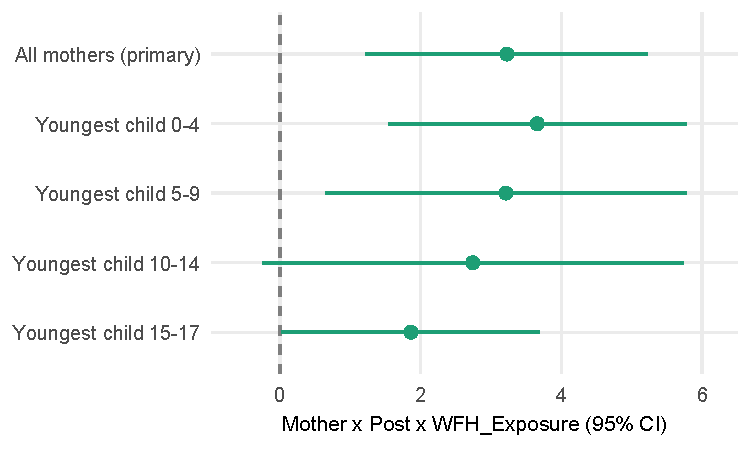
\includegraphics[width=0.75\textwidth]{../outputs/figures/hours_ddd_by_child_age.pdf}
\caption{Hours DDD triple interaction by age of the youngest child}\label{fig:childage}
\begin{minipage}{0.8\textwidth}\small
\vspace{0.3em}
\emph{Notes:} The DDD column of Table~\ref{tab:childage}: $\Mother \times \Post \times \WFH$
with 95\% confidence intervals clustered by occupation, one estimate per youngest-child age bin,
each against all childless women. The top row is the pooled estimate of Table~\ref{tab:hours}.
\end{minipage}
\end{figure}

\subsection{Heterogeneity by population group, and the fathers' comparison}\label{sec:res-subgroup}

Table~\ref{tab:subgroup} re-estimates the hours DiD and DDD separately for Jewish and Arab women,
and on men as a comparison population. For Jewish women the pattern is the pooled pattern: the DiD is $0.3021$
(SE $0.2027$), indistinguishable from zero, while the DDD is $2.8465$\sym{**} (SE $0.9125$). For
Arab women the DiD is $-0.0724$ (SE $0.4785$), also indistinguishable from zero --- and Arab
women's hours fell in the post-period overall ($\Post = -2.162$\sym{***}) --- while the DDD is
$5.5069$\sym{*} (SE $2.6741$), nominally significant and nearly twice the Jewish point estimate.
Neither group shows an average effect; both show an exposure gradient.

We do not read the larger Arab estimate as evidence that the mechanism is stronger for Arab women.
The two coefficients are not statistically distinguishable: the Arab subsample is about nine times
smaller ($24{,}307$ versus $209{,}727$ occupation-matched women with observed hours), its standard
error nearly three times larger, and a two-sample $z$-test on the DDD term gives $z = 0.942$,
$p = 0.346$. There is also a mechanical reason for the imprecision: Arab women's employment in
Israel is concentrated in a narrow set of occupations, disproportionately education and health-aide
roles, so comparatively few two-digit occupations carry enough Arab respondents to inform an
occupation-specific comparison, and a small number of high-leverage occupations can dominate the
estimate. The Arab result is therefore best described as imprecisely estimated and statistically
indistinguishable from the Jewish estimate --- a thin-coverage fragility rather than a documented
heterogeneous treatment effect.

The fathers' comparison is a comparison, not a placebo, and has to be read on both margins.
Re-estimating the same models on men, with ``mother'' read as ``father,'' gives a DiD of
$-0.4002$\sym{*} (SE $0.1883$, $N = 261{,}543$) and a DDD of $-1.7620$ (SE $1.0153$,
$N = 251{,}779$), the latter negative and significant at the $10\%$ level. Fathers in
teleworkable occupations are exposed to remote work exactly as mothers are, so a null was never
the prediction; what the comparison shows is that the exposure gradient has the opposite sign for
fathers, and that the two gradients are statistically distinguishable ($z = 3.461$, $p = 0.0005$).
A macro trend common to all workers in teleworkable jobs cannot produce a positive gradient for
mothers alongside a negative one for fathers, which rules out the most obvious confound; and a
negative gradient for fathers is what within-household reallocation would look like if mothers'
additional paid hours in teleworkable jobs were matched by fathers' additional care hours. We
report that as a substantive reading the data are consistent with, not as a result, since the
design is not built to identify it. The falsification test proper is
Section~\ref{sec:res-falsification}.

On the plain DiD fathers' hours fall by $0.40$ relative to childless men, a larger and more
significant movement than the $0.23$ we estimate for mothers, and although the two are
distinguishable ($z = 2.406$, $p = 0.016$) the difference is driven by the fathers' coefficient.
We do not claim an average effect for mothers on that margin; Section~\ref{sec:res-did} reads the
female DiD as a null, and the fathers' comparison is consistent with that reading.

\begin{table}[htbp]
\centering
\begin{threeparttable}
\caption{Hours DiD and DDD by subgroup, and the fathers' comparison}\label{tab:subgroup}
\renewcommand{\baselinestretch}{1}\footnotesize
\setlength{\tabcolsep}{3pt} % seven columns; at \small the default 6pt overran the text width
\begin{tabular}{lcccccc}
\toprule
 & \multicolumn{3}{c}{DiD: $\Mother \times \Post$} & \multicolumn{3}{c}{DDD: $\Mother \times \Post \times \WFH$} \\
\cmidrule(lr){2-4}\cmidrule(lr){5-7}
Subgroup & Coef. & SE & $N$ & Coef. & SE & $N$ \\
\midrule
All women (primary) & $0.2280$ & $0.1809$ & 251{,}857 & $3.224$\sym{**} & $1.022$ & 246{,}326 \\
Jewish women & $0.3021$ & $0.2027$ & 214{,}449 & $2.847$\sym{**} & $0.9125$ & 209{,}727 \\
Arab women & $-0.0724$ & $0.4785$ & 24{,}975 & $5.507$\sym{*} & $2.674$ & 24{,}307 \\
Men (fathers vs.\ childless) & $-0.4002$\sym{*} & $0.1883$ & 261{,}543 & $-1.762$\sym{\cdot} & $1.015$ & 251{,}779 \\
\midrule
95\% CI, Jewish & \multicolumn{3}{c}{$[-0.0952,\ 0.6994]$} & \multicolumn{3}{c}{$[1.0579,\ 4.6351]$} \\
95\% CI, Arab & \multicolumn{3}{c}{$[-1.0103,\ 0.8656]$} & \multicolumn{3}{c}{$[0.2657,\ 10.7481]$} \\
Jewish vs.\ Arab, $z$ ($p$) & \multicolumn{3}{c}{$0.720$ (0.471)} & \multicolumn{3}{c}{$-0.942$ (0.346)} \\
Women vs.\ men, $z$ ($p$) & \multicolumn{3}{c}{$2.406$ (0.016)} & \multicolumn{3}{c}{$3.461$ (0.001)} \\
\bottomrule
\end{tabular}

\begin{tablenotes}\small
\item Weekly hours, reference-week workers, standard controls. DiD clustered by individual; DDD
clustered by occupation. Men: ``Mother'' read as ``Father,'' a comparison population rather than
a placebo (Section~\ref{sec:diagnostics}). Two-sample $z$-tests as described there. Confidence
intervals use the normal critical value. \autonoteSubgroup
\end{tablenotes}
\end{threeparttable}
\end{table}

\subsection{The extensive margin, briefly}\label{sec:res-extensive}

The employment margin is where this sample has the least room to move --- mothers' employment rate
exceeds childless women's in the raw data --- and it is secondary for a reason of power that is
worth stating once. Column~(1) of Table~\ref{tab:extensive} reports equation~\eqref{eq:did} with
employment as the outcome: $\Mother \times \Post = -0.0053$ (SE $0.0052$). The mother/non-mother
employment gap did not change after the shift to remote work, and the estimate is precise --- its
standard error is about half a percentage point --- so this is an informative null. Employment rose
in the post-period for all women ($\Post = 0.0153$\sym{***}); the DiD estimated separately for
Jewish and Arab women is $-0.0041$ (SE $0.0058$) and $-0.0208$ (SE $0.0138$), neither significant;
and the pre-period event-study coefficients pass their joint test ($F(2, 79{,}069) = 0.63$,
$p = 0.53$).

Column~(2) reports the employment DDD with the cell-based exposure index. The triple interaction is
$-0.0257$ (SE $0.0725$); a variant with fully interacted age-by-education-by-district cell fixed
effects gives $-0.0194$ (SE $0.0722$). This null is of a different kind. At $\alpha = 0.05$ and
80\% power the design could detect a triple interaction no smaller than $0.2031$ per unit of
exposure --- and the cell-based index never moves a unit: its standard deviation on the estimation
sample is $0.0706$ and its interquartile range $0.0766$, so the detectable effect is $1.43$
percentage points per standard deviation of exposure, or $1.85\%$ of the baseline employment rate
of $0.7737$. Against the closest published benchmark, \citeauthor{harrington2025}'s $0.78$
percentage points per 10\% rise in WFH, the design is underpowered by a factor of about two to
three. The shortfall is structural --- a binary outcome and a regressor with a standard deviation
of $0.07$ --- and re-clustering, combining the two margins into a single outcome, and refining the
exposure-cell partition did not close it. The employment DDD is therefore \emph{uninformative}: it
is evidence neither for nor against a WFH-mediated employment effect, and the two nulls in
Table~\ref{tab:extensive} should not be read as one verdict. The one significant coefficient,
$\Post \times \WFH = -0.1555$\sym{**}, indicates a general post-2021 employment decline in
high-exposure cells that is unrelated to motherhood. This is what motivates the intensive-margin
design, where occupation-level exposure is available.

\begin{table}[htbp]
\centering
\begin{threeparttable}
\caption{Extensive margin: employment DiD and DDD}\label{tab:extensive}
\renewcommand{\baselinestretch}{1}\small
\begin{tabular}{lcc}
\toprule
 & (1) DiD & (2) DDD, cell-based exposure \\
\midrule
Mother $\times$ Post $\times$ WFH\_Exposure &  & $-0.0257$ \\
 &  & $(0.0725)$ \\
Mother $\times$ Post & $-0.0053$ & $0.0065$ \\
 & $(0.0052)$ & $(0.0168)$ \\
Mother $\times$ WFH\_Exposure &  & $-0.1404$\sym{\cdot} \\
 &  & $(0.0803)$ \\
Post $\times$ WFH\_Exposure &  & $-0.1555$\sym{**} \\
 &  & $(0.0566)$ \\
WFH\_Exposure &  & $0.0131$ \\
 &  & $(0.0565)$ \\
Mother & $-0.0034$ &  \\
 & $(0.0041)$ &  \\
Post & $0.0153$\sym{***} &  \\
 & $(0.0043)$ &  \\
Constant & $0.4926$\sym{***} &  \\
 & $(0.0085)$ &  \\
\midrule
MDE ($\alpha=0.05$, power $0.80$), per unit &  & $0.2031$ \\
MDE per SD of exposure &  & $0.0143$ \\
\quad as \% of baseline employment rate &  & 1.85\% \\
\midrule
Observations & 364{,}784 & 355{,}984 \\
$R^2$ & 0.227 & 0.221 \\
Clustering & individual & demographic cell ($\approx 210$) \\
\bottomrule
\end{tabular}

\begin{tablenotes}\small
\item Dependent variable: employment indicator; full sample of employed and non-employed women.
Standard controls in both columns; column (2) adds Mother $\times$ age-group interactions, so its
Mother and Post main effects are not separately reported. Column (2) uses the demographic-cell
shift-share index of Section~\ref{sec:exposure}, whose standard deviation on this sample is
$0.0706$ and interquartile range $0.0766$; the per-unit MDE therefore answers a question the data
cannot pose, and the per-SD row is the interpretable one. Baseline employment rate $0.7737$.
\autonoteExtensive
\end{tablenotes}
\end{threeparttable}
\end{table}

%======================================================================
\section{Discussion}\label{sec:discussion}
%======================================================================

Among mothers who remain in work, there is no post-2021 hours effect on average. There is a large
one in teleworkable occupations. Those two statements are the paper's result, and it is the
conjunction that makes it informative: a triple-interaction coefficient of about $3.2$ additional
weekly hours per unit of exposure, an implied change at zero exposure that is if anything negative,
and a selection correction the estimate survives. This is consistent with WFH access relaxing a
binding time constraint specifically for mothers in teleworkable jobs --- the \citet{goldin2014}
mechanism --- and it is difficult to reconcile with a general post-pandemic recovery common to all
women, which would have raised hours across occupations rather than only where the work can be done
from home. Fathers show the opposite gradient, and the gradient is steepest for mothers of the
youngest children.

How precisely the effect is estimated is a separate question from whether it is there, and the
paper keeps the two apart. The exposure score varies across forty occupations, and the three
procedures that take that seriously do not agree: the analytic standard error puts the estimate
at the $1\%$ level, the permutation test at $5\%$, the wild cluster bootstrap at $10\%$. The
pattern of evidence --- a saturated specification that changes nothing, a top-quartile contrast
significant on its own, a monotone child-age gradient, an opposite-signed fathers' gradient and a
selection correction that barely moves the bounds --- is what makes the finding credible; no
single $p$-value does.

Which occupations are doing the work is concrete. The calibration step moved ten occupations away
from their US task-based scores toward realized Israeli behavior: clerical support and teaching
were corrected sharply downward, because Israeli institutional practice kept them in person
regardless of task content, while ICT professionals remained high on both measures. The triple
interaction is identified off exactly this contrast, which grounds ``exposure'' in checkable
occupational content. That the raw external index yields a positive but insignificant estimate is
consistent with that reading, and the check of Section~\ref{sec:res-robust} that drops the ten
calibrated occupations altogether --- and finds a larger estimate on the thirty that remain ---
shows the calibration is not what produces the result.

The magnitude is economically meaningful where it applies. For a mother at the top quartile's
mean exposure the regression implies a post-2021 change of about $1.4$ hours a week
($-0.54 + 3.22 \times 0.59$), and the raw top-quartile difference-in-differences of
Figure~\ref{fig:dose-response} is $1.55$; the difference between the top and bottom quartiles is
$1.7$ hours by the regression and $1.9$ by the raw cell means. Set against the $1.74$-hour
intensive-margin penalty of Table~\ref{tab:hours}, mothers in the most teleworkable jobs recovered
roughly four fifths of the penalty after 2021, and mothers in the least teleworkable jobs
recovered none of it. The size is also what the most literal form of the time-constraint mechanism would produce:
\citet{aksoy2023} put the commuting time saved at about 72 minutes per day worked from home, so two
remote days a week free roughly two and a half hours, and a mother who returns most of that time
to paid work is a mother whose hours rise by about the amount estimated here.

The timing is also informative. The event study rises gradually from an insignificant 2021 estimate
to a significant one in 2023, consistent with WFH adoption and household time reallocation being a
multi-year adjustment rather than an instantaneous response to the 2020--21 shock. The 2023
coefficient is the largest on both margins, and Section~\ref{sec:limitations} notes a reason to
hold that year's estimate a little more loosely than the others.

Why hours and not employment? The employment DDD is not a failed test of the mechanism; it is an
uninformative one, underpowered by a factor of two to three against the closest published effect.
The intensive-margin design is better powered because it can use occupation-level exposure, which
the employment design cannot without conditioning its own outcome on itself. Substantively, the two
results are coherent: the effect operates on \emph{how much} mothers in teleworkable jobs work, not
on \emph{whether} they are employed, which is precisely the margin \citet{kleven2019denmark}
identify as a leading channel of the child penalty. This is also where our findings depart from
\citet{harrington2025}: their US evidence is on employment and income, and we cannot confirm or
reject an employment effect in Israel with this design. The policy reading is correspondingly
narrow: WFH availability matters for how intensively mothers who already hold \emph{teleworkable}
jobs can work, not for whether mothers in general hold jobs or how much they work --- which is where
our evidence speaks, and where it does not.

The subgroup results are more modest than the point estimates suggest. The Jewish-women estimate
carries the pooled result. The Arab-women estimate is larger but imprecise, statistically
indistinguishable from the Jewish one, and rests on thin occupational coverage; we report it
transparently but do not claim heterogeneity on its basis. The one heterogeneity we do read
substantively is by the age of the youngest child, because the mechanism predicts its direction
in advance: the gradient is twice as large for mothers of under-fives as for mothers of
teenagers, which is what a time constraint that binds through child care should produce.

%======================================================================
\section{Limitations}\label{sec:limitations}
%======================================================================

\paragraph{Parallel trends.}
Joint pre-trend tests do not reject on either margin, nor does the triple difference's own
(Figures~\ref{fig:pretrend} and~\ref{fig:pretrend-ddd}). The last is the test that matters for
the headline estimate and, as Section~\ref{sec:res-ddd-diag} explains, the one with the least
power: it is evidence of no visible violation, not proof of none.

\paragraph{The narrowed hours estimand.}
Hours are usual hours among women who were working, not among all women holding a job, and roughly
$10\%$ of each year's employed sample is excluded on that basis. The exclusion is not innocuous for
the triple interaction if absence from work is itself related to WFH exposure, and it is: absence
runs at $14.4\%$ of the employed in the least teleworkable quartile of occupations against
$8.5$--$9.6\%$ in the other three, and among mothers it fell after 2021 in the top quartile while
rising in the bottom one.\footnote{Reference-week absence among employed women aged 25--59 with a
matched occupation, by the quartiles of Figure~\ref{fig:dose-response}: $14.4\%$, $8.5\%$, $9.5\%$
and $9.6\%$ from the least to the most teleworkable quartile. Among mothers the top-quartile share
fell from $12.1\%$ to $10.4\%$ after 2021 and the bottom-quartile share rose from $15.5\%$ to
$16.9\%$; among childless women the top-quartile share is $6.1\%$ in both periods.} Movement across
the absence margin is therefore part of what selection into the observed-hours sample means here,
which is why the bounds of Section~\ref{sec:lee} define selection on that sample rather than on
employment. They trim it; they do not assume it away.

\paragraph{Lee bounds: direction and monotonicity.}
The trimming construction handles only \emph{excess} selection in the post-period mother cell ---
the direction the hypothesis predicts --- and not under-selection, which is a missing-data problem
rather than an excess-observed-data one. It assumes monotone selection to justify trimming from a
single tail, and computes selection rates unweighted, consistent with the rest of the analysis.
Small excess selection means the construction found little to correct, not that the selection
concern is absent.

\paragraph{Survey weights.}
CBS survey weights are intentionally not applied in any outcome regression. This is a scope
decision, not an oversight: reported rates and coefficients are unweighted estimates on the analysis
sample, not population-representative statistics. The one exception is internal to constructing
the cell-based exposure index, where occupation exposure is aggregated to demographic cells using
the survey weight; that is not a representativeness correction for the outcome regressions.

\paragraph{Exposure is partly post-treatment.}
Neither exposure measure that delivers a significant estimate is fully pre-treatment: the
calibrated index draws on 2022--23 realized WFH for its swap test, and the realized index is
anchored to 2021 because no 2020 extract exists. Section~\ref{sec:res-robust} gives the reasons
the calibration is unlikely to manufacture the result; the fully pre-treatment external index
nonetheless yields a positive and insignificant estimate, and a reader who weights that measure
more heavily than we do will read the headline as directionally supported rather than established.
The crosswalk behind the external index is itself undocumented (Section~\ref{sec:exposure}).

\paragraph{The 2023 survey year.}
The 2023 coefficient is the largest in both event studies, and the 2023 survey year includes the
quarter in which the war that began on 7 October 2023 disrupted the labor market: mass reserve
call-ups, which bear on men's hours and so on the fathers' comparison, and school closures and evacuations,
which bear on mothers'. The timing reading of Section~\ref{sec:discussion} does not rest on 2023
alone, since 2021 and 2022 are individually significant on the triple difference, and the estimate
survives dropping the year (Section~\ref{sec:res-robust}); the 2023 point should nonetheless be
held more loosely than the others. Early 2021 likewise included a third lockdown with partial
school closure, so the post-period is ``post-acute'' more cleanly in its later years than in its
first.
% The exclusion is of the whole year: the survey-month field (ChodeshSeker) is dropped at cleaning,
% so a fourth-quarter-only exclusion would need a schema change (audit item I5).

\paragraph{Who is childless.}
The control group is any woman aged 25--59 with no child under 17 in the household, so it includes
women whose children are grown and women who become mothers within the window;
\citet{harrington2025}'s design shares this feature. If part of the control group responds to the
treatment as mothers do, the DiD is biased toward zero, against the effect we report rather than
for it. The treatment group is correspondingly broad, from mothers of infants to mothers of
sixteen-year-olds; Section~\ref{sec:res-childage} splits it by the youngest child's age.

\paragraph{Age controls and age imbalance.}
Age enters as a categorical age-group code, because the extract has no continuous age or
birth-year variable. Mothers and non-mothers are imbalanced on this code in the pre-period, and the
imbalance tracks exposure quartile; the age-interacted and reweighted specifications address it
and the estimate survives, but the reweighted attenuation ($3.224 \to 2.597$) is the largest
single move any check produces, so the result is robust to age imbalance in direction and
approximate magnitude, not insensitive to it.

\paragraph{Exposure is measured coarsely, and on a mixed scale.}
Exposure is assigned at the two-digit occupation level, forty groups, and \citet{buzaglo2023}
shows that within-firm sorting matters as much as occupation for Israeli gender gaps. The
calibrated score also mixes task-based probabilities for thirty occupations with realized
shares for ten, and Section~\ref{sec:exposure} shows that this costs cross-sectional fit: the
raw external index predicts realized remote work better in levels. A score on a single scale
--- realized shares for every occupation --- is the realized index of Table~\ref{tab:robust},
which gives a larger and noisier estimate; whether to make it primary is a design choice we
flag rather than settle here.
Within-occupation heterogeneity in teleworkability is classical measurement error in the
regressor, which attenuates the triple interaction toward zero, so the estimate is if anything a
lower bound on the effect of actual teleworkability. Occupation codes masked by the CBS for
disclosure control are dropped when building exposure; a proxy check finds no strong evidence of
bias from this, though that evidence is weak.

\paragraph{Inference.}
The hours DDD clusters on forty occupation groups, and the three procedures of
Section~\ref{sec:res-robust} disagree on the headline's significance level: $1\%$ on the
analytic standard error, $5\%$ under the permutation test, $10\%$ under the wild cluster
bootstrap. That range, not the analytic $p$-value, is the paper's statement of how precisely the
effect is estimated. The panel does not support within-person identification: only 1.9\% of
respondents span the pre/post boundary.

%======================================================================
\section{Conclusion}\label{sec:conclusion}
%======================================================================

% =====================================================================================
% SKELETON -- NOT SUBMITTABLE TEXT. REPLACE THIS ENTIRE BLOCK WITH YOUR OWN PROSE.
%
% The assignment requires this section to be written individually by the student
% (paper/archive/old_paper.tex:209-213). What follows is a five-paragraph structure with the
% claims each paragraph can rest on, in note form, with the section where each is established.
% Target 400-500 words and at most three numbers in the prose. Write your own sentences from it.
%
% The previously-committed model answer was removed on 2026-09-19. If you want it back for
% self-comparison it is in git history: `git show d662aa3^:paper/paper.tex`.
%
% Every figure below was verified against a committed artifact during the pre-submission
% audit (see docs/pre-submission-audit-decisions.md). Delete this whole block, banner and
% all, once your text is in, and drop \usepackage{xcolor} with it.
% =====================================================================================
\noindent\textbf{\color{red}[SKELETON ONLY --- REPLACE WITH YOUR OWN TEXT BEFORE SUBMISSION]}

\begin{enumerate}\itshape\small
\item \textbf{Paragraph 1 --- the question and the move.} \citet{harrington2025} for the US; this
paper takes it to Israel \emph{and} to hours conditional on working. Not a replication
(Sections~\ref{sec:lit}, \ref{sec:data}).

\item \textbf{Paragraph 2 --- the result as a conjunction.} No average effect: the hours DiD is
$0.2280$ (SE $0.1809$), a reasonably precise null that the selection correction widens rather
than overturns. An effect confined to teleworkable work: the triple interaction is $3.224$
(SE $1.022$, $p<0.01$), survives the generalized correction (Imbens--Manski $[1.021, 5.324]$) and
two age-balance specifications, and at zero exposure the implied change is negative. Fathers show
no exposure gradient, and the women/men difference is $z = 3.461$
(Sections~\ref{sec:res-did}--\ref{sec:res-subgroup}).

\item \textbf{Paragraph 3 --- what it means.} Goldin's time-constraint mechanism: the response is
where the work can be done from home, and nowhere else. A result about \emph{which} mothers
benefit, not about mothers as a group. Measurement is part of it: the mechanism is visible only
once exposure is measured as Israeli jobs were actually done (Section~\ref{sec:discussion}).

\item \textbf{Paragraph 4 --- what the design cannot say.} Employment: the DiD is a precise null,
the DDD is uninformative (MDE $1.43$ percentage points per SD of exposure, two to three times the
Harrington benchmark), and the two should not be conflated. Earnings: not observed. The calibrated
exposure is partly post-treatment; the 2023 year includes the war; inference rests on forty
clusters; estimates are unweighted (Sections~\ref{sec:res-extensive}, \ref{sec:limitations}).

\item \textbf{Paragraph 5 --- policy reading and next steps.} WFH availability bears on how
intensively mothers already employed in teleworkable jobs work, not on whether mothers are
employed. Next: an earnings outcome, which needs income data linked to the survey since the
extract carries none; a higher-powered test of the employment margin; a jointly estimated model
letting the mechanism differ by sex and population group.
\end{enumerate}

\noindent\textbf{\color{red}[END SKELETON --- DELETE THIS BLOCK]}

%======================================================================
\bibliographystyle{apalike}
\bibliography{references}

%======================================================================
\appendix
\setcounter{table}{0}\renewcommand{\thetable}{A\arabic{table}}
\setcounter{figure}{0}\renewcommand{\thefigure}{A\arabic{figure}}
\section{Appendix: the occupation-level exposure scores}\label{sec:appendix-exposure}
%======================================================================

Table~\ref{tab:exposure-scores} lists, for each of the forty two-digit ISCO-08 occupations, the
external \citet{dingel2020} score, the realized share usually working from home in 2022--23 that
the calibration of Section~\ref{sec:exposure} tests it against, whether the score was swapped,
the calibrated score the hours DDD uses, and the realized share working from home in the
reference week over 2021--23 on men and women pooled. Figure~\ref{fig:first-stage} plots the
last of these against the calibrated score. The ten swapped occupations sit above the 45-degree
line, because their calibrated value is the usual-place share, which is lower than the
reference-week share for every occupation; the thirty unswapped ones lie below it, most of them
far below, which is the visual form of the scale-mixing Section~\ref{sec:exposure} describes.
The five unswapped occupations with calibrated scores above $0.5$ (science and engineering
professionals; legal, social and cultural professionals and their associate professionals; ICT
technicians; numerical and material recording clerks) have realized reference-week shares
between $0.15$ and $0.38$, all below the swapped ICT professionals at $0.62$. The
correlations and slopes quoted there (calibrated: $0.53$ and $0.40$ against the reference-week
share, $0.48$ and $0.26$ against the usual-place share; external: $0.74$ and $0.37$, and $0.59$
and $0.21$) are computed on these forty points, with the slope weighted by the pooled employed
sample in each occupation.

\begin{table}[htbp]
\centering
\begin{threeparttable}
\caption{External, realized and calibrated WFH exposure by two-digit occupation}\label{tab:exposure-scores}
\renewcommand{\baselinestretch}{1}\scriptsize
\setlength{\tabcolsep}{3pt}
\begin{tabular}{lp{5.2cm}cccccc}
\toprule
ISCO & Occupation (ISCO-08 sub-major group) & Ext. & Real.\ 22--23 & Swap & Calib. & Ref.-wk 21--23 & $N$ \\
\midrule
11 & Chief executives and legislators & 0.900 & 0.155 & yes & 0.155 & 0.320 & 2{,}855 \\
12 & Administrative and commercial managers & 0.892 & 0.143 & yes & 0.143 & 0.336 & 3{,}859 \\
13 & Production and specialised services managers & 0.638 & 0.097 & yes & 0.097 & 0.199 & 9{,}990 \\
14 & Hospitality, retail and other services managers & 0.773 & 0.066 & yes & 0.066 & 0.132 & 2{,}827 \\
21 & Science and engineering professionals & 0.644 & 0.210 &  & 0.644 & 0.349 & 13{,}228 \\
22 & Health professionals & 0.101 & 0.059 &  & 0.101 & 0.088 & 9{,}665 \\
23 & Teaching professionals & 0.966 & 0.069 & yes & 0.069 & 0.184 & 20{,}496 \\
24 & Business and administration professionals & 0.943 & 0.233 & yes & 0.233 & 0.449 & 10{,}479 \\
25 & ICT professionals & 1.000 & 0.360 & yes & 0.360 & 0.615 & 14{,}638 \\
26 & Legal, social and cultural professionals & 0.678 & 0.215 &  & 0.678 & 0.371 & 13{,}344 \\
31 & Science and engineering associate professionals & 0.144 & 0.059 &  & 0.144 & 0.106 & 3{,}926 \\
32 & Health associate professionals & 0.057 & 0.080 &  & 0.057 & 0.084 & 2{,}203 \\
33 & Business and administration associate professionals & 0.684 & 0.123 & yes & 0.123 & 0.223 & 22{,}415 \\
34 & Legal, social and cultural associate professionals & 0.577 & 0.142 &  & 0.577 & 0.206 & 5{,}480 \\
35 & ICT technicians & 0.750 & 0.244 &  & 0.750 & 0.380 & 2{,}491 \\
41 & General and keyboard clerks & 1.000 & 0.098 & yes & 0.098 & 0.144 & 4{,}846 \\
42 & Customer services clerks & 0.292 & 0.096 &  & 0.292 & 0.159 & 3{,}875 \\
43 & Numerical and material recording clerks & 0.526 & 0.071 &  & 0.526 & 0.152 & 4{,}948 \\
44 & Other clerical support workers & 0.625 & 0.083 & yes & 0.083 & 0.161 & 1{,}049 \\
51 & Personal service workers & 0.271 & 0.146 &  & 0.271 & 0.144 & 7{,}808 \\
52 & Sales workers & 0.200 & 0.050 &  & 0.200 & 0.063 & 8{,}704 \\
53 & Personal care workers & 0.300 & 0.046 &  & 0.300 & 0.045 & 17{,}206 \\
54 & Protective services workers & 0.100 & 0.008 &  & 0.100 & 0.011 & 3{,}969 \\
61 & Market-oriented skilled agricultural workers & 0.182 & 0.027 &  & 0.182 & 0.051 & 1{,}325 \\
62 & Market-oriented skilled forestry, fishery and hunting workers & 0.179 & 0.000 &  & 0.179 & 0.045 & 22 \\
63 & Subsistence farmers, fishers, hunters and gatherers & 0.000 & 0.375 &  & 0.000 & 0.375 & 8 \\
71 & Building and related trades workers & 0.027 & 0.008 &  & 0.027 & 0.016 & 5{,}208 \\
72 & Metal, machinery and related trades workers & 0.000 & 0.008 &  & 0.000 & 0.013 & 3{,}982 \\
73 & Handicraft and printing workers & 0.138 & 0.118 &  & 0.138 & 0.129 & 666 \\
74 & Electrical and electronic trades workers & 0.000 & 0.022 &  & 0.000 & 0.042 & 3{,}424 \\
75 & Food, wood, garment and other craft workers & 0.073 & 0.122 &  & 0.073 & 0.109 & 2{,}304 \\
81 & Stationary plant and machine operators & 0.000 & 0.019 &  & 0.000 & 0.017 & 2{,}407 \\
82 & Assemblers & 0.000 & 0.012 &  & 0.000 & 0.015 & 1{,}166 \\
83 & Drivers and mobile plant operators & 0.237 & 0.006 &  & 0.237 & 0.006 & 8{,}480 \\
91 & Cleaners and helpers & 0.000 & 0.004 &  & 0.000 & 0.003 & 3{,}474 \\
92 & Agricultural, forestry and fishery labourers & 0.000 & 0.007 &  & 0.000 & 0.016 & 192 \\
93 & Labourers in mining, construction, manufacturing and transport & 0.120 & 0.006 &  & 0.120 & 0.008 & 2{,}659 \\
94 & Food preparation assistants & 0.000 & 0.013 &  & 0.000 & 0.011 & 649 \\
95 & Street and related sales and service workers & 0.000 & 0.000 &  & 0.000 & 0.043 & 23 \\
96 & Refuse workers and other elementary workers & 0.250 & 0.022 &  & 0.250 & 0.024 & 493 \\
\bottomrule
\end{tabular}

\begin{tablenotes}\footnotesize
\item Ext.: the \citet{dingel2020} teleworkability score at the two-digit ISCO-08 level, via
the crosswalk described in Section~\ref{sec:exposure}. Real.\ 22--23: share of employed
respondents (men and women, all ages in the extract) who usually work from home in 2022--23,
the calibration's benchmark; Swap: the calibration replaced the external score with it.
Calib.: the score the hours DDD uses. Ref.-wk 21--23: share who worked from home in the survey
reference week over 2021--23, men and women pooled, with $N$ the pooled employed sample carrying
that item. Codes 1--3 (armed forces) carry no external score and are not in the sample.
\end{tablenotes}
\end{threeparttable}
\end{table}

\begin{figure}[htbp]
\centering
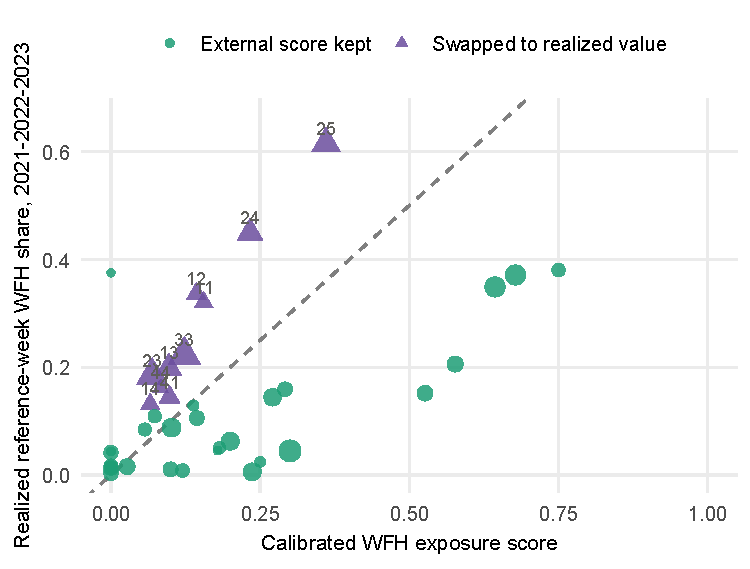
\includegraphics[width=0.8\textwidth]{../outputs/figures/wfh_first_stage_occupation.pdf}
\caption{First stage: calibrated exposure score against realized reference-week WFH, by
occupation}\label{fig:first-stage}
\begin{minipage}{0.8\textwidth}\small
\vspace{0.3em}
\emph{Notes:} One point per two-digit occupation, sized by the pooled employed sample in
2021--23; triangles are the ten occupations the calibration swapped to their realized value,
labelled by ISCO-08 code. The dashed line is the 45-degree line. Statistics in the text of
Section~\ref{sec:exposure}.
\end{minipage}
\end{figure}

\end{document}
